\documentclass[twoside,11pt]{article}
\usepackage[preprint]{jmlr2e}
\usepackage{times}
\usepackage{amsmath,mathtools,booktabs,microtype,enumitem}
\usepackage{lastpage}
\hypersetup{hidelinks,
pdftitle={Certifying Prediction Limits and Representation Refinement with Kernel Affine Hull Machines},
pdfauthor={Mohit Kumar and Somayeh Kargaran},
pdfsubject={KAHM forecasting, representation refinement, and finite-sample risk certification}}
\jmlrheading{}{2026}{1--\pageref{LastPage}}{}{}{}{Mohit Kumar and Somayeh Kargaran}
\ShortHeadings{Prediction Limits and Representation Refinement}{Kumar and Kargaran}
\firstpageno{1}
\allowdisplaybreaks
\setlength{\emergencystretch}{1.5em}

\begin{document}
\title{Certifying Prediction Limits and Representation Refinement\\with Kernel Affine Hull Machines}
\author{\name Mohit Kumar \email mohit.kumar@uni-rostock.de\\
\addr University of Rostock, Rostock, Germany\\
Software Competence Center Hagenberg, Hagenberg, Austria
\AND
\name Somayeh Kargaran \email somayeh.kargaran@scch.at\\
\addr Software Competence Center Hagenberg, Hagenberg, Austria}
\maketitle

\begin{abstract}
Can a representation support a prescribed forecasting accuracy, and is a
more expensive representation necessary? We study these questions using
Kernel Affine Hull Machine (KAHM) features and sensitivity-constrained decoders.
A pairwise lower bound measures target separations that exceed the decoder's
Lipschitz budget. We characterize its slack, establish sharp cases, and exhibit
arbitrarily loose cases. Stratifying pairs while preserving the marginal risk
can recover missed obstructions. Finite-sample bounds account for estimated
stratum masses and combine with fitted-risk upper bounds to certify acceptance,
exclusion, or minimum feasible representation cost among predefined classes.
Retained feature blocks with a sum-of-block-norms budget preserve earlier
predictors and prevent exact duplication from enlarging the class. Experiments
compare the witness with range-aware variance and empirical-minimum-risk bounds;
the latter is often tighter. A controlled forecasting study demonstrates
additional cost and infeasibility decisions, with substantial sample requirements.
Six synthetic systems, pen trajectories, and speech energy
illustrate the forecasting procedure. KAHM gains depend on the task and decoder;
conventional regressors remain stronger on several tasks. Speech calibration
certifies selected tolerances under an explicit independent-group assumption.
All guarantees concern expected squared error under a specified evaluation law.
\end{abstract}
\begin{keywords}
Kernel Affine Hull Machines, time-series forecasting, soft state abstraction,
representation refinement, prediction risk certification
\end{keywords}

\section{Introduction}
\label{sec:introduction}

Kernel Affine Hull Machines (KAHMs) describe data using geometric reconstruction
models in reproducing kernel Hilbert spaces
\citep{kumar2024kahm,kumar2025collaborative}. Applied to time-series histories,
their reconstruction affinities give soft associations with learned reference
groups. This offers a concrete way to build a forecasting representation:
local models describe the histories, their associations form a dictionary, and
a decoder predicts the observed future signal. The central question is whether
that geometry preserves distinctions that matter for prediction. Histories
with almost identical associations may have different futures, and a larger
dictionary need not improve a forecast learned from finite data.

Reconstruction quality and prediction of the soft coordinates do not answer
that question. A coordinate-space objective changes when the dictionary changes;
even a collapsed representation can have a small latent prediction error. We
therefore keep the future observed output as the target throughout learning,
refinement, and evaluation. For horizon $h$ and tolerance $\epsilon_h$, we ask
whether a fitted KAHM forecast has population root-mean-square error at most
$\epsilon_h$, and whether the representation can support that accuracy within
a prescribed decoder sensitivity class. Both questions refer to the same law
for new trajectories and forecast origins.

This paper extends the KAHM research program from geometric modeling and
soft-state prediction limits to an implemented forecasting procedure.
\citet{kumar2026limits} study norm-bounded linear prediction of successor soft
coordinates, separate exact Koopman closure from empirical fitting, and give
KAHM constructions. That work also includes fitted-model upper risk bounds and
independent-trajectory evaluation. We retain the KAHM reconstruction mechanism
and that sampling principle. The extensions here are a fixed raw-output
prediction task, a directly estimable pairwise obstruction for Lipschitz
decoders, refinement that preserves earlier forecasts, and a calibrated
decision procedure for fitted accuracy and actual refinement gains.

The obstruction has a simple geometric interpretation. If two future targets
are separated by more than the decoder's sensitivity times the distance between
their representations, the two prediction errors cannot both be small.
Averaging a squared positive-part discrepancy over conditionally independent
copies lower-bounds prediction risk. Its comparison with a variance obstruction
uses the same pairing law: pairing at a common forecast origin and pairing
within a reference class are different constructions.

Refinement also requires a consistent meaning of model capacity. Replacing a
KAHM dictionary need not retain its earlier predictors. We instead append
dictionary blocks, use a sum of block coefficient norms, and match that budget
to the maximum distance across blocks. An old forecast remains feasible by
setting new coefficients to zero. Exact duplicates can be merged without
increasing the budget, so replication alone cannot improve the population
optimum or the obstruction. A genuinely new block may help, and its fitted
benefit is assessed separately on independent data.

The contributions are as follows.
\begin{enumerate}[leftmargin=*,itemsep=3pt]
\item \textbf{A KAHM forecasting learner.} We combine stable soft reconstruction
affinities, retained KAHM dictionaries, and convex constrained multihorizon
decoders to predict the original output. The complete procedure freezes its
candidates before calibration and can return an unresolved accuracy decision.
\item \textbf{Matched lower and upper risk statements.} We derive a pairwise
obstruction for arbitrary Lipschitz decoders, establish its relation to a
conditional variance bound and its exactness on a two-atom law, and combine it
with fitted-risk certificates for independent episodes.
\item \textbf{Comparable refinement.} We establish nested, replication-invariant
prediction classes and a necessary amount of geometric change for a refinement
to meet a tolerance. Paired losses assess actual fitted improvements; the
population nesting result does not guarantee that every fitted refinement helps.
\item \textbf{An empirical assessment of KAHM design choices.} Retained
experiments compare soft and hard associations, direct prediction and feature
rollout, dictionary sizes, decoder budgets, and input preprocessing. The study
adds matched KAHM, RBF, and affine-hull comparisons across three heads with
equal preprocessing and dictionary-size options on all seven tasks. It
separates accuracy, representation cost, certificate usefulness, and variation
across fitting repetitions, retaining gains and regressions.
\end{enumerate}

KAHMs provide the principal geometric construction; the risk and refinement
arguments apply more generally to representations satisfying the stated
assumptions. This permits comparison with alternative geometric dictionaries
under a common forecasting and evaluation procedure. The guarantee concerns
expected squared error for a new episode and a prescribed origin law. It does
not assert sufficient-state discovery, exact Koopman closure, conditional
prediction-interval coverage, or validity for arbitrary windows from a single
dependent trajectory.

\section{Related work}
\label{sec:related}

\paragraph{Geometric representations and Koopman prediction.}
KAHMs learn reconstruction models in reproducing kernel Hilbert spaces
(RKHSs) \citep{kumar2024kahm,kumar2025collaborative}. We use these established
reconstruction models to construct forecasting features.
Soft state aggregation \citep{singh1994soft}, approximate state abstraction
\citep{abel2016abstraction}, and task-oriented latent transition models
\citep{gelada2019deepmdp} likewise distinguish a representation from its
predictive use. Extended dynamic mode decomposition approximates Koopman
operators on finite dictionaries \citep{williams2015edmd}; learned dictionaries
\citep{li2017dictionary} and RKHS regression bounds \citep{kostic2022regression}
provide related forecasting frameworks. Basis-invariant consistency diagnostics
\citep{haseli2023consistency}, multistep projection-error guarantees and
refinement \citep{conradie2026trustworthy}, and residual-based dictionary
learning \citep{coote2026residual} address dictionary quality. Our decisions
instead compare expected observed-output error with a declared tolerance
while preserving a common target and sampling law.

\paragraph{Closest KAHM prediction-limit analysis.}
The earlier analysis of \citet{kumar2026limits}, in its cited third version, provides
class-centered lower certificates, empirical-minimum comparisons, fitted-risk
upper bounds, and independent evaluation. It also gives an exact four-state
example and independent dynamical confirmation. We reuse its KAHM
construction and sampling principle; neither certificates for KAHM nor
independent confirmation is new here. Table~\ref{tab:prior-comparison}
states the substantive differences. Their reconstruction-score margin bounds
concern agreement with reference labels, which does not imply predictive
sufficiency.

\begin{table}[t]
\centering\small
\begin{tabular}{@{}p{0.19\linewidth}p{0.35\linewidth}p{0.40\linewidth}@{}}
\toprule
Question & \citet{kumar2026limits} & Present work \\
\midrule
Prediction target & Successor soft coordinates & Fixed observed future outputs \\
Decoder class & Spectral-norm-bounded linear coordinate predictors & General Lipschitz oracle; retained-block affine fits \\
Lower information & Class-centered variation; empirical-minimum comparator & Positive-part pair slack; normalized monotone block hierarchy \\
Representation decisions & Accuracy exclusion for a fixed coordinate map and norm limit & Simultaneous class exclusion and fitted-model acceptance; minimum feasible cost among declared alternatives \\
\bottomrule
\end{tabular}
\caption{Scope relative to arXiv:2609.32652v3. KAHM reconstruction,
independent evaluation, and standard concentration are shared foundations.
The scalar block consistency result requires the conditions in
Theorem~\ref{thm:block-hierarchy}.}
\label{tab:prior-comparison}
\end{table}

\paragraph{Pairwise bounds and Lipschitz regression.}
\citet{akash2021inverse} derive a Lipschitz-constrained mean squared error (MSE) bound
using paired residuals and target separation. Their argument is a close
antecedent to the geometric step in our witness; our contribution concerns
its conditional positive-part form, sharpness and slack, and statistically
valid stratification under the unchanged marginal risk. Finite-support
Lipschitz regression can be posed as a constrained optimization problem
\citep{gottlieb2017regression}; we use this class directly for an empirical-minimum
comparator. Model-class falsification \citep{muller2025falsification} and
minimal-empirical-risk bounds \citep{wu2026minimal} provide broader context.
The Gamma test uses local pair differences to estimate regression noise
\citep{evans2002gamma}. Lipschitz set-membership identification
\citep{milanese2004setmembership}, trajectory invalidation
\citep{jin2020invalidation}, and corruption-robust prediction ranges
\citep{blum2026reliable} concern related feasibility questions with different
sampling and error criteria.

\paragraph{Empirical minima and optimization over blocks.}
Expected sample-average optimization values and repeated-batch lower bounds
are established in stochastic programming
\citep{linderoth2006empirical,guigues2017confidence}. Optimization of empirical
$U$-statistics and the tradeoff between computation and statistical precision
are also established \citep{clemencon2016scaling}. Our block objective can be
written as the minimum of a residual-difference $U$-statistic. We do not claim
that empirical-minimum lower bounds or block averaging are new. The specific
connection is a centered hierarchy for scalar Lipschitz regression: its
size-two member is the pair witness, its expectations increase to the class
optimum under compactness, and exact examples quantify why a fixed block size
can remain inadequate. The recentering argument uses closure under adding
constants; the pair formula and scalar extension connect it to the Lipschitz
prediction problem. Calibration uses standard bounded-mean inequalities.

\paragraph{Calibration, refinement, and dependence.}
We use classical bounded-mean inequalities \citep{hoeffding1963} and empirical
Bernstein and standard-deviation bounds \citep{maurer2009empirical}. The
simultaneous testing principle follows Learn then Test
\citep{angelopoulos2025ltt}. Our group norm is established in group selection
and multiple-kernel learning \citep{bach2008group}; here its max-block dual
metric gives a comparable sensitivity budget as dictionaries grow. Soft gating
and residual fitting also have established precedents
\citep{jordan1994experts,buhlmann2003boosting}. The additional cost conclusion
comes from jointly excluding cheaper classes and accepting a fitted model.

Within-episode dependence is allowed because concentration is applied to
independent episode summaries. A chronological split of one dependent record
does not provide that independence. Forecasting bounds under other sampling
assumptions \citep{mcdonald2017forecasting} and dependence-aware conformal
analysis \citep{oliveira2024conformal} illustrate the additional conditions
needed; their guarantees are not consequences of the present theorem.

\section{Learning a certified soft-state forecasting model}
\label{sec:method}

\subsection{A fixed raw-output forecasting task}

Let $y_t\in\mathbb R^d$ be an observed time series. A causal history is
$x_t=(y_{t-m+1},\ldots,y_t)$, optionally augmented by covariates available at
time $t$. For a finite set of horizons $\mathcal H$, the target is
$Y_t=(y_{t+h}:h\in\mathcal H)$. The history length, target transformation,
forecast origins, and horizons are part of the task definition. When comparing
different history lengths, we use the same origins, starting only after the
longest history is available. This prevents a change in evaluation law from
being confused with a change in model quality.

The main implementation fits direct forecasts at each requested horizon, sharing
the geometric representation and a joint coefficient budget. This is a
conditional time-series prediction model; it need not be a generative model for
entire trajectories. Direct fitting avoids relying on an unverified relation
between one-step feature error and the distribution encountered during a long
rollout. Iterated feature-transition models are included as separate baselines
and evaluated on exactly the same raw targets.

Development, validation, calibration, and test episodes have distinct roles.
Training estimates feature maps and decoder coefficients. Validation can choose
ordinary hyperparameters or identify one representative per model family.
Calibration supplies the confidence statements and may select among the entire
family frozen before it is observed. The final test set is used only to describe
forecasting behavior independently of those decisions. A test estimate is not
treated as an exact population risk.

\subsection{Geometric dictionaries and stable soft associations}

For dictionary block $b$, partition the training histories into $C_b$ reference
groups and fit one KAHM reconstruction model to each group, following
\citet{kumar2024kahm,kumar2025collaborative,kumar2026limits}. Let
$T_{bc}(x)\in[0,1]$ denote the resulting folding score. With fixed positive
$\omega$ and $\tau$, define
\begin{equation}
 \Phi_{bc}(x)=
 \frac{(1-T_{bc}(x)+\tau)^\omega}
 {\sum_{r=1}^{C_b}(1-T_{br}(x)+\tau)^\omega},
 \qquad \Phi_b(x)\in\Delta_{C_b}.
 \label{eq:soft-features}
\end{equation}
The implementation evaluates this expression by subtracting the maximum
log-affinity before exponentiation. A small positive denominator is not replaced
by a uniform vector. The latter operation changes the representation and can
destroy meaningful relative weights even when they are representable in log
arithmetic. A unit test contains a concrete case where the direct powers sum to
less than $10^{-12}$ but one normalized association is essentially one.

The original repository's KAHM training and folding routines are reused, with
their source hashes retained in the experiment manifest. In the original
experimental campaigns, history standardization uses training moments only.
The separate follow-up in Section~\ref{sec:input-scaling} compares this
preprocessing with training-only range scaling and bounded raw histories.
Geometry-fitting input subsampling and the maximum
number of local training points are fixed in the configuration. The resulting
maps are then held fixed when subsequent decoder fits and calibration are
performed.

Retain the stack $\Gamma_s(x)=(\Phi_1(x),\ldots,\Phi_s(x))$. Each block lies in
a simplex; the concatenation lies in a product of simplices. Different blocks
need not have nested cluster partitions. It is the retention of their actual
coordinate functions that preserves the old forecast class. Our experiments
use $C_b\in\{2,4,8,16\}$, so the four retained feature dimensions are
$2,6,14,30$.

\subsection{A constrained multihorizon decoder}

Collect the horizon targets as rows of a matrix $Y$. For a retained stack with
training feature matrix $F=[F_1,\ldots,F_s]$, fit
\begin{equation}
 \min_{a,W}\ \frac1N\|Y-\mathbf1a^\top-FW\|_{\rm F}^2
                   +\lambda\|W\|_{\rm F}^2
 \quad\text{subject to}\quad
                \sum_{b=1}^s\|W_b\|_{\rm F}\leq\kappa.
 \label{eq:training-objective}
\end{equation}
Here $W_b$ contains the rows associated with block $b$ and all output horizons;
the intercept is unpenalized. We use row-vector notation in
\eqref{eq:training-objective}; the equivalent column-vector decoder in the
theory section transposes these matrices. The complete prediction is the
coordinatewise projection of $a+W^\top\Gamma_s(x)$ onto the task's known
output box. The objective is convex before output clipping. The clipping step
is used at prediction time and is included in every reported loss.

Centering eliminates the intercept. Projected accelerated gradient then solves
the constrained quadratic. Projection is inexpensive: compute the Frobenius
norm of each coefficient block, project that nonnegative vector onto an
$\ell_1$ ball of radius $\kappa$, and rescale the blocks. The implementation
records a convex first-order optimality gap, not merely the change between
successive iterates. Appendix~\ref{app:optimization} gives the projection and
gap derivations. Accurate optimization is useful for interpreting the learner;
the held-out fitted-risk certificate remains valid even if the solver stops
early, provided the returned coefficient budget is feasible.

The ridge term is a numerical and statistical regularizer, whereas the block
constraint defines the sensitivity class. Exact replication leaves the
constrained class unchanged, but splitting coefficients over duplicate blocks
can change a squared-Frobenius ridge penalty. Replication-invariance claims below
concern feasible prediction classes and the obstruction. A separate zero-ridge
numerical test checks equality of duplicate and nonduplicate optimum risks
within their reported optimization gaps.

\subsection{Calibration and model selection}

Algorithm~\ref{alg:procedure} describes the implemented finite-family procedure.
The candidate collection includes history lengths, dictionary prefixes,
geometric feature types, and baselines. A representation-specific lower bound
and fitted-model upper bound use the same raw target, origin law, and decoder
sensitivity budget. An upper bound for the raw signal is never paired with a
lower bound for a different latent-coordinate target.

\begin{figure}[t]
\centering
\fbox{\begin{minipage}{0.94\linewidth}
\textbf{Algorithm 1: Certified geometric forecasting}
\begin{enumerate}[leftmargin=*,itemsep=3pt]
\item Specify horizons, causal origins, known target bounds, tolerances,
confidence level, and a candidate-cost rule.
\item On development data, fit geometric blocks, retain their prefixes, and
fit constrained decoders. Fit the comparison models on the same raw targets.
\item Freeze the entire candidate family, preprocessing, sensitivity budgets,
and any proposed refinement comparisons.
\item On new independent episodes, compute one averaged squared loss per
episode and horizon. Pair episodes disjointly and compute target-distance
obstruction scores at corresponding origins.
\item Allocate the failure probability over all requested risk statements and
improvement comparisons. Compute simultaneous lower and upper endpoints.
\item Return the least costly candidate whose upper endpoints meet all
tolerances. Also report excluded classes and inconclusive candidates. If no
candidate passes, return an unresolved decision.
\end{enumerate}
\end{minipage}}
\caption{The finite-family learner and its certification decision. A new model
fitted after inspecting calibration requires fresh evaluation data or a
separately justified adaptive guarantee.}
\label{alg:procedure}
\end{figure}

The lower endpoint can justify expanding the representation or changing the
sensitivity budget, but cannot prove that a proposed modification helps. We
therefore additionally compare old and new fitted forecasts through paired
episode losses. The procedure can certify an actual improvement even when the
class obstruction is zero. Conversely, it may exclude a restricted class even
if no tested refinement attains the desired accuracy.

In the numerical study, model cost is the number of retained feature
coordinates, with fixed tie-breaking by history length and validation error.
This is a transparent representation-size proxy, not an inference-runtime
measurement. For a deployment with unequal feature-evaluation costs, the same
selection theorem permits any cost function fixed before calibration.

\section{Pairwise obstructions and certified forecasting}
\label{sec:theory}

This section separates three questions: whether a representation can support a
specified accuracy, whether a fitted forecaster attains that accuracy, and what
can be concluded when the representation is refined.  All population risks
refer to the same raw forecasting target.  No Markov assumption, invariant
distribution, or exact Koopman closure is imposed.

\subsection{A directly estimable pairwise obstruction}

Let $X$ be an available history, $Y\in\mathbb R^q$ a future target, and
$U=\Gamma(X)$ a fixed representation.  Let $d$ be a pseudometric on the
representation space and write
\[
 \mathcal G_\kappa(d)
 =\{g:\|g(u)-g(v)\|_2\leq\kappa d(u,v)\},\qquad
 R^*_\kappa(\Gamma,d)=\inf_{g\in\mathcal G_\kappa(d)}
             \mathbb E\|Y-g(U)\|_2^2.
\]
The metric, representation, and nonnegative budget $\kappa$ are fixed before
the certificate data are observed.  The infimum may be over a larger class
than the fitted decoder family.  A lower bound for this larger class is also
a lower bound for every decoder in the family.

For a conditioning variable $A$, construct $(U,Y)$ and $(U',Y')$ independently
conditional on $A$, with the same conditional law and with the original
marginal law for each copy.  The case of a constant $A$ is an ordinary
independent pair.  Define
\begin{equation}
 W_{\kappa,A}(\Gamma,d)
 =\frac12\mathbb E\left[
       \bigl(\|Y-Y'\|_2-\kappa d(U,U')\bigr)_+^2\right].
 \label{eq:pair-witness}
\end{equation}
The shared variable specifies a sampling construction; arbitrary nearest
neighbor matching is not covered by this definition.

\begin{theorem}[Pairwise prediction obstruction]
\label{thm:pair-obstruction}
Assume $\mathbb E\|Y\|_2^2<\infty$.  Then
\begin{equation}
 R^*_\kappa(\Gamma,d)\geq W_{\kappa,A}(\Gamma,d).
 \label{eq:pair-population}
\end{equation}
For Euclidean representation distance, assume also $\mathbb E\|U\|_2^2<\infty$ and put
\[
 \sigma_{Y\mid A}^2=\mathbb E\|Y-\mathbb E[Y\mid A]\|_2^2,
 \qquad
 \tau_{U\mid A}^2=\mathbb E\|U-\mathbb E[U\mid A]\|_2^2.
\]
Then the pairwise obstruction satisfies
\begin{equation}
 W_{\kappa,A}(\Gamma,\|\cdot\|_2)
 \geq (\sigma_{Y\mid A}-\kappa\tau_{U\mid A})_+^2.
 \label{eq:pair-dominance}
\end{equation}
Both comparisons use the same conditioning variable and evaluation law.
\end{theorem}

\begin{proof}
Fix an admissible $g$ with finite risk and set $r=Y-g(U)$ and
$r'=Y'-g(U')$.  The triangle inequality and the Lipschitz condition give
\[
 (\|Y-Y'\|_2-\kappa d(U,U'))_+\leq\|r-r'\|_2.
\]
Conditional independence gives
\[
 \mathbb E[\|r-r'\|_2^2\mid A]
 =2\{\mathbb E[\|r\|_2^2\mid A]
                    -\|\mathbb E[r\mid A]\|_2^2\}.
\]
Taking expectations proves $W_{\kappa,A}\leq R(g)$; taking the infimum
proves \eqref{eq:pair-population}.  Infinite-risk predictors satisfy the
inequality trivially.  To prove \eqref{eq:pair-dominance}, write
$a=\|Y-Y'\|_2$ and $b=\|U-U'\|_2$.  Pointwise,
$a\leq(a-\kappa b)_++\kappa b$.  The triangle inequality in $L^2$ therefore
implies
\[
 \|(a-\kappa b)_+\|_{L^2}
 \geq(\|a\|_{L^2}-\kappa\|b\|_{L^2})_+
 =\sqrt2(\sigma_{Y\mid A}-\kappa\tau_{U\mid A})_+.
\]
Square and divide by two.
\end{proof}

The new statistic estimates a squared positive-part distance discrepancy
directly.  It does not estimate two variances separately and then subtract
their square roots.  This distinction can matter when retained input
variation is small.  It is not a claim of a new minimax estimation rate:
bounded-mean concentration is used below, and taking a square root of a
risk bound can still have slow behavior near zero.  In particular,
\eqref{eq:pair-dominance} does not imply that pairing at a common time origin
dominates a certificate conditioned on a different reference class $c(X)$.

\begin{proposition}[Exactness on a two-atom law]
\label{prop:two-atom}
Let $(U,Y)$ equal $(u_0,y_0)$ with probability $p\in(0,1)$ and
$(u_1,y_1)$ otherwise.  Use Euclidean input distance and an unconditioned
independent pair.  Then
\begin{equation}
 R^*_\kappa
 =W_\kappa
 =p(1-p)\bigl(\|y_1-y_0\|_2
                 -\kappa\|u_1-u_0\|_2\bigr)_+^2.
 \label{eq:two-atom-optimum}
\end{equation}
The optimum is attainable by an affine map.  If the outputs are constrained
to a closed convex set containing $y_0,y_1$, projecting that map onto the
set preserves the optimum and the Lipschitz budget.
\end{proposition}

\begin{proof}
Let $q=1-p$, $a=\|y_1-y_0\|_2$, $b=\|u_1-u_0\|_2$, and
$\mu=py_0+qy_1$.  The two unequal ordered pairs have total probability
$2pq$, so \eqref{eq:pair-witness} gives the right side of
\eqref{eq:two-atom-optimum} as a lower bound.  If $a=0$, a constant predictor
attains zero.  Otherwise let $v=(y_1-y_0)/a$ and $s=\min\{a,\kappa b\}$.
Choose fitted values $f_0=\mu-qsv$ and $f_1=\mu+psv$.  Their separation is
$s$, and their risk is $pq(a-s)^2$.  If $b=0$, these values coincide and
a constant map attains this risk.  If $b>0$, the affine map
\[
 g(u)=f_0+
 \frac{\langle u-u_0,u_1-u_0\rangle}{b^2}(f_1-f_0)
\]
has operator norm $s/b\leq\kappa$ and the prescribed two fitted values.
Both fitted values lie on the segment between $y_0$ and $y_1$.  Euclidean
projection onto a closed convex output set fixes these values and is
nonexpansive.
\end{proof}

\subsection{Independent episodes, dependent observations within episodes}

Let $E_1,\ldots,E_n$ be independent, identically distributed complete
episodes, independent of all model construction and selection data.  For
horizon $h$, let $\mathcal T_h$ be a fixed nonempty set of available causal
origins common to all episodes and all compared candidates.  Within an
episode, observations may have arbitrary dependence and their distribution
may change with time.  Candidate $j$ has a representation $\Gamma_j$,
metric $d_j$, frozen forecaster $f_{jh}=g_{jh}\circ\Gamma_j$, and known
Lipschitz budget $\kappa_{jh}$ for its decoder.  Denote its episode loss by
\begin{equation}
 Z_{i,jh}=\frac1{|\mathcal T_h|}\sum_{t\in\mathcal T_h}
       \|Y_{i,t+h}-f_{jh}(X_{i,t})\|_2^2,
 \qquad R_{jh}=\mathbb E Z_{i,jh}.
 \label{eq:episode-risk}
\end{equation}
This is risk for a new episode and a uniformly sampled common origin.  It
is not a guarantee conditional on each particular history.  Different
episode weights or a different origin law define a different risk.

Assume the target and prediction lie in a known closed convex output set
of diameter $D_h$, and put $B_h=D_h^2$.  Prediction clipping alone is
insufficient if the target is unbounded.  Bounds inferred only from observed
training minima and maxima do not establish the assumed population range.
For $m=\lfloor n/2\rfloor$ disjoint episode pairs define
\begin{equation}
 Q_{r,jh}=\frac1{2|\mathcal T_h|}\sum_{t\in\mathcal T_h}
 \left(\|Y_{2r-1,t+h}-Y_{2r,t+h}\|_2
 -\kappa_{jh}d_j(\Gamma_j(X_{2r-1,t}),
                         \Gamma_j(X_{2r,t}))\right)_+^2.
 \label{eq:episode-pairs}
\end{equation}
The $Z_i$ are independent across episodes, and the $Q_r$ are independent
across disjoint pairs.  The terms within either average need not be
independent.  Their ranges are $[0,B_h]$ and $[0,B_h/2]$, respectively.
For the pair statistic, the conditioning variable in
Theorem~\ref{thm:pair-obstruction} is the common random origin $A=t$.

For observations $V_1,\ldots,V_N$ in an interval of length $b$, let
$\bar V$ be their mean and $s_V^2=(N-1)^{-1}\sum_i(V_i-\bar V)^2$.
For $N\geq2$ define
\begin{equation}
 \operatorname{rad}_{\rm EB}(V;b,\alpha)
 =\sqrt{\frac{2s_V^2\log(2/\alpha)}{N}}
       +\frac{7b\log(2/\alpha)}{3(N-1)}.
 \label{eq:eb-radius}
\end{equation}
This is the bounded-variable empirical Bernstein radius of
\citet{maurer2009empirical}; applying it to the reflected variables gives
the lower confidence bound used here.

\begin{theorem}[Simultaneous two-sided episode certificate]
\label{thm:episode-certificate}
Suppose $J$ candidates and $H$ horizons are frozen using independent
development data, $n\geq4$, and all fitted decoders satisfy their stated
Lipschitz budgets.  Set $\alpha=\delta/(2JH)$ and
\begin{align}
 L_{jh}&=\max\{0,\bar Q_{jh}
 -\operatorname{rad}_{\rm EB}(Q_{\cdot,jh};B_h/2,\alpha)\},
 \label{eq:pair-lcb}\\
 U_{jh}&=\min\{B_h,\bar Z_{jh}
 +\operatorname{rad}_{\rm EB}(Z_{\cdot,jh};B_h,\alpha)\}.
 \label{eq:risk-ucb}
\end{align}
With probability at least $1-\delta$, conditional on the development data,
all $j,h$ simultaneously satisfy
\begin{equation}
 L_{jh}\leq W_{jh}\leq R^*_{jh}\leq R_{jh}\leq U_{jh}.
 \label{eq:risk-sandwich}
\end{equation}
Here $R^*_{jh}$ is the minimum risk over all $\kappa_{jh}$-Lipschitz
decoders of $\Gamma_j$ under the same horizon, origin law, and raw target.
\end{theorem}

\begin{proof}
Condition on development data.  For each fixed $j,h$, apply the empirical
Bernstein inequality to the $n$ episode losses and its reflected version
to the $m$ disjoint-pair scores.  A union bound over the $2JH$ events gives
simultaneous validity with failure probability at most $\delta$.
Theorem~\ref{thm:pair-obstruction}, applied at each common origin and
averaged over origins, gives $W_{jh}\leq R^*_{jh}$.  The fitted decoder
belongs to the infimum's class, giving $R^*_{jh}\leq R_{jh}$.  Independence
between the upper and lower statistics is not required.
\end{proof}

The confidence parameter $\delta$ controls the random calibration sample.
It does not state that every future error is at most $\sqrt U$, or give
conditional coverage of a prediction interval.  The effective independent
sample sizes in \eqref{eq:eb-radius} are $n$ and $m$, not the number of
overlapping windows.  More origins can reduce the variability of an
episode average, but cannot be counted as additional independent episodes.
The representation, score normalization, dictionary sizes, budgets,
horizons, and any baseline included in the reported joint event must all
be fixed before calibration.  Training-dependent choices are allowed
because the guarantee conditions on training.

\begin{corollary}[Acceptance, exclusion, and inconclusive decisions]
\label{cor:decisions}
On the event in \eqref{eq:risk-sandwich}, $U_{jh}\leq\epsilon_h^2$
certifies that the fitted forecaster attains root-mean-square error at
most $\epsilon_h$.  The inequality $L_{jh}>\epsilon_h^2$ excludes that
tolerance for every decoder in the corresponding Lipschitz class.
When neither condition holds, the decision is inconclusive.  Among a
frozen finite family, selecting any candidate satisfying
$U_{jh}\leq\epsilon_h^2$ at every required horizon preserves these
guarantees.  In particular, a predeclared cost can be minimized over the
certified candidates, with abstention if the set is empty.
\end{corollary}

The selected candidate is cheapest among those certified by the data,
not necessarily among all candidates whose unknown true risks meet the
tolerance.  Also, $\sqrt{U_{jh}}-\sqrt{L_{jh}}$ upper-bounds the fitted
decoder's RMSE suboptimality within the stated class, but a large gap
does not diagnose optimization error: the lower witness and both
confidence corrections can be loose.

For transparent sample-size calculations, the empirical Bernstein radii
can instead be replaced by the prespecified Hoeffding radii
$b\sqrt{\log(1/\alpha)/(2N)}$.  If a fitted risk is at least $\gamma>0$
below a squared-error tolerance, $n\geq
2B_h^2\log(1/\alpha)/\gamma^2$ makes its Hoeffding upper bound pass
that tolerance with probability at least $1-\alpha$.  Similarly, if a
pair-witness mean exceeds the tolerance by $\gamma$, then
$m\geq B_h^2\log(1/\alpha)/(2\gamma^2)$ makes the corresponding lower
bound exclude it with probability at least $1-\alpha$.  These statements
follow by bounding the empirical mean's deviation in the direction
opposite to the confidence bound.  They are sufficient sample sizes,
not optimal rates, and use the witness margin rather than the unknown
oracle-risk margin for exclusion.  Taking the better of separately
computed Hoeffding and empirical Bernstein bounds requires a joint
confidence allocation or a single prespecified choice.

\subsection{Refinement that preserves the meaning of the norm budget}

Let $\Phi_1,\ldots,\Phi_s$ be simplex-valued geometric dictionaries, with
possibly different numbers of coordinates, and retain the whole stack
$\Gamma_s=(\Phi_1,\ldots,\Phi_s)$.  Refinement appends a block; it does
not silently refit or replace previous blocks.  Use the block maximum
metric and the sum of block Frobenius norms,
\begin{equation}
 d_s(x,x')=\max_{1\leq b\leq s}
                  \|\Phi_b(x)-\Phi_b(x')\|_2,
 \qquad
 \|W\|_{2,1}=\sum_{b=1}^s\|W_b\|_{\rm F}.
 \label{eq:block-geometry}
\end{equation}
The notation $d_s$ denotes the induced pseudometric on histories, or
equivalently the block maximum metric on the stacked representation.
The decoder class is
\begin{equation}
 \mathcal F_{s,\kappa}
 =\left\{x\mapsto\Pi_{\mathcal Y}\!
       \left(a+\sum_{b=1}^sW_b\Phi_b(x)\right):
                         \sum_b\|W_b\|_{\rm F}\leq\kappa\right\},
 \label{eq:block-decoder}
\end{equation}
where the intercept $a$ is unpenalized and $\Pi_{\mathcal Y}$ is
Euclidean projection onto the convex output set.  Group norm constraints
are established tools \citep{bach2008group}; their role here is to align retained geometric
blocks with the sensitivity budget used in the certificate.

\begin{theorem}[Nested and replication-invariant refinement]
\label{thm:replication-invariance}
Every decoder in $\mathcal F_{s,\kappa}$ is $\kappa$-Lipschitz with
respect to $d_s$.  Appending a block preserves
$\mathcal F_{s,\kappa}\subseteq\mathcal F_{s+1,\kappa}$, and
$d_{s+1}\geq d_s$ pointwise.  Consequently, the optimal risk in the
decoder class cannot increase, and the population pair witness cannot
increase at the same $\kappa$ and with the same pairing law.  Appending
an exact copy of an existing block leaves both the decoder class and
the pair witness unchanged.
\end{theorem}

\begin{proof}
For the unprojected decoder,
\[
 \left\|\sum_bW_b\bigl(\Phi_b(x)-\Phi_b(x')\bigr)\right\|_2
 \leq\sum_b\|W_b\|_{\rm F}
                  \|\Phi_b(x)-\Phi_b(x')\|_2
 \leq\kappa d_s(x,x').
\]
Projection is nonexpansive, so the same bound holds afterward.  Set a
new block's coefficient to zero to embed any old decoder in the refined
class.  The maximum distance increases when a new block is added;
therefore each positive-part pair score decreases or stays unchanged.
If the new block duplicates block $b$, its contribution can be merged
into $W_b$ and
$\|W_b+W_{s+1}\|_{\rm F}\leq\|W_b\|_{\rm F}+
\|W_{s+1}\|_{\rm F}$.  This proves reverse inclusion of the decoder
classes.  A duplicate does not change a maximum distance.
\end{proof}

The risk statement concerns population optima in nested feasible sets,
not the performance of separately fitted finite-sample estimators.
Nor does it imply that every newly learned block supplies useful
information.  The maximum metric remains bounded by $\sqrt2$ because
each block is simplex-valued; its range does not grow merely by adding
blocks.  If a fitted decoder's smaller actual norm is used for an
additional certificate, that changes the comparator class.  Monotonicity
across refinements is claimed only at a common norm budget.

This distinction is material for a usual Frobenius constraint on the
concatenated coefficient matrix.  Consider a two-point input with
$\Phi(x_0)=e_1$, $\Phi(x_1)=e_2$, equally likely targets $-1$ and $1$,
and budget one.  Its best affine MSE is
$(2-\sqrt2)^2/4$.  Duplicating the block permits coefficients
$(-1/2,1/2,-1/2,1/2)$ of Frobenius norm one and zero error.  No information
was added: duplication only relaxed the effective norm constraint.
The block-sum construction prevents this effect.  It does not prevent
a genuinely different block from changing the useful geometry.

\begin{theorem}[A necessary amount of geometric change]
\label{thm:necessary-expansion}
Let $d_0,d_1$ be two induced representation pseudometrics on the same
histories, and use the same target, conditionally independent pairing
law, and positive sensitivity budget $\kappa$.  Write
$\Delta=(d_1(X,X')-d_0(X,X'))_+$ and let $W_0,W_1$ be their pair
witnesses.  Then
\begin{equation}
 \sqrt{W_1}\geq
 \left(\sqrt{W_0}-\frac{\kappa}{\sqrt2}
                       \|\Delta\|_{L^2}\right)_+.
 \label{eq:metric-change}
\end{equation}
In particular, if any $\kappa$-Lipschitz decoder of the new
representation attains RMSE at most $\epsilon$, then
\begin{equation}
 \|\Delta\|_{L^2}\geq
       \frac{\sqrt2}{\kappa}(\sqrt{W_0}-\epsilon)_+.
 \label{eq:required-change}
\end{equation}
On any event $L_0\leq W_0$, replacing $W_0$ by $L_0$ in the right side
of \eqref{eq:required-change} is valid simultaneously for every new
representation.  The new representations need not have been fixed
when $L_0$ was computed.
\end{theorem}

\begin{proof}
Let $a=\|Y-Y'\|_2$ and $v_i=(a-\kappa d_i)_+$.  The hinge function is
nonexpansive, and pointwise $v_0\leq v_1+\kappa\Delta$.
Consequently $\|v_1\|_{L^2}\geq
(\|v_0\|_{L^2}-\kappa\|\Delta\|_{L^2})_+$, which proves
\eqref{eq:metric-change}.  A feasible new decoder with RMSE at most
$\epsilon$ implies $W_1\leq\epsilon^2$ by
Theorem~\ref{thm:pair-obstruction}; rearrange.  The final statement
follows from the deterministic inequality and monotonicity in $W_0$.
\end{proof}

This is a necessary condition, not a sufficient refinement rule.  It
rules out repairs whose pairwise distance expansion is too small.  The
quantity $L_0$ must lower-bound the old \emph{pair witness}; an arbitrary
lower bound on old oracle risk cannot be substituted.  If sensitivity
budgets are also changed, the corresponding necessary condition is
\[
 \| (\kappa_1d_1-\kappa_0d_0)_+\|_{L^2}
 \geq\sqrt2(\sqrt{W_{\kappa_0,0}}-\epsilon)_+.
\]
This form makes explicit that increasing sensitivity can compensate for
changing the geometry.

\subsection{When an added block can improve prediction}

The preceding obstruction only identifies a necessary geometric change.
The following elementary quadratic-risk calculation identifies a
sufficient population condition for a particular residual direction.
It is a projection calculation, not a claim that a positive obstruction
guarantees a useful split.

\begin{proposition}[Residual correlation and budget slack]
\label{prop:residual-gain}
Consider the unprojected affine decoder
\[
 f_0(x)=a+\sum_{b=1}^sW_b\Phi_b(x),
\]
with $\sum_b\|W_b\|_{\rm F}<\kappa$, and let
$\psi(X)\in\mathbb R^p$ be a new square-integrable feature block.
Write
\[
 r=Y-f_0(X),\quad C=\mathbb E[r\psi(X)^\top],\quad
 G=\mathbb E[\psi(X)\psi(X)^\top],\quad
 s_0=\kappa-\sum_b\|W_b\|_{\rm F}.
\]
If $C\ne0$, define $a_0=\|C\|_{\rm F}^2$,
$b_0=\operatorname{tr}(CGC^\top)$, and
\[
 \eta=\min\{a_0/b_0,\ s_0/\sqrt{a_0}\}.
\]
Then $b_0>0$, the appended coefficient $V=\eta C$ is feasible, and
\begin{equation}
 R(f_0)-R(f_0+V\psi)
       =2\eta a_0-\eta^2b_0\geq\eta a_0>0.
 \label{eq:residual-gain}
\end{equation}
If $f_0(X)$ already lies in the convex output set almost surely,
projecting the new forecast onto that set retains this improvement.
\end{proposition}

\begin{proof}
Expanding the square gives
$R(f_0+V\psi)=R(f_0)-2\langle V,C\rangle_{
m F}
+\operatorname{tr}(VGV^\top)$.  For $V=\eta C$ this yields the equality
in \eqref{eq:residual-gain}.  The budget holds because
$\|V\|_{
m F}=\eta\sqrt{a_0}\leq s_0$.  If $b_0=0$, then
$C\psi=0$ almost surely.  For each row $c$ of $C$ this implies
$c\psi=0$ almost surely, whence
$\|c\|_2^2=\mathbb E[r_\ell\psi^\top]c^\top
=\mathbb E[r_\ell(c\psi)]=0$, contradicting $C\ne0$.
Since $\eta\leq a_0/b_0$, the gain is at least $\eta a_0$.
Projection onto a convex set containing $Y$ cannot increase squared
error; when $f_0$ is already in the set, its reference risk is unchanged.
\end{proof}

The proviso about the old output is essential.  Improvement of two
unprojected affine risks does not, by itself, imply improvement between
their separately clipped versions.  Nor does the proposition guarantee
strict improvement when the old decoder exhausts its budget.  For
actual clipped models, improvement is checked directly using paired
episode losses.  The moments in Proposition~\ref{prop:residual-gain} are
population moments: substituting estimates from training does not by
itself retain the claimed population gain.

For two forecasts fixed before an independent evaluation block, define
$D_i=Z_i^{\rm old}-Z_i^{\rm new}\in[-B_h,B_h]$.  With probability at
least $1-\alpha$,
\begin{equation}
 R^{\rm old}-R^{\rm new}\geq
 \bar D-\operatorname{rad}_{\rm EB}(D;2B_h,\alpha).
 \label{eq:paired-improvement}
\end{equation}
A positive right side certifies actual risk reduction for the two
fitted predictors.  A nonpositive value is inconclusive.  To certify
many fixed comparisons jointly, allocate confidence over the whole
comparison family.  For genuinely adaptive sequential refinement,
each new candidate may depend on the past, but its evaluation block
must be fresh and independent conditional on that past.  Assigning
stage failure probabilities $\alpha_s$ with
$\sum_s\alpha_s\leq\delta$ and accepting a change only when its
paired lower bound is positive then makes every accepted improvement
valid on a common event of probability at least $1-\delta$.  This
follows by conditional validity at each stage and a union bound; it
does not authorize repeatedly tuning on one fixed calibration set.

Finally, a positive obstruction need not be repairable.  If $Y$ is an
independent, symmetric random sign of amplitude $a$, then every
representation measurable from $X$ has Bayes risk $a^2$.  A constant
representation already has pair witness $a^2$; no refinement of the
observed history can remove this independent future noise.  Conversely,
a zero pair witness is not proof of a useful predictor.  Matched-origin
pairing, for example, sees no variation between identical deterministic
episodes even if an inadequate representation loses variation between
origins.  These examples motivate reporting obstruction, fitted risk,
and inconclusive outcomes separately.

\section{Lower-bound comparisons beyond two atoms}
\label{sec:witness-comparison}

The two-atom law in Proposition~\ref{prop:two-atom} has an exact population witness. We now
separate population slack from calibration error on eight fixed finite laws
(Table~\ref{tab:witness-laws}), including deterministic targets, noise,
partial collapse, rare conflicts, and an affine--Lipschitz class mismatch.
For every method, $R^*$ is the minimum MSE over the same full scalar
$1$-Lipschitz class with outputs in $[-1,1]$. This is a certificate comparison,
not another KAHM forecasting benchmark.

\begin{table}[t]
\centering\footnotesize
\setlength{\tabcolsep}{3pt}
\begin{tabular}{llll}
\toprule
Law & Representation values $u_i$ & Targets $y_i$ & Stratum labels $c(u_i)$ \\
\midrule
Collapsed binary & $(0,0)$ & $(-1,1)$ & $(0,0)$ \\
Two atoms & $(-.6/\sqrt2,.6/\sqrt2)$ & $(-1,1)$ & $(0,0)$ \\
Three-point V & $(-1,0,1)$ & $(1,-1,1)$ & $(0,0,1)$ \\
Five-point zigzag & $(-1,-.5,0,.5,1)$ & $(-1,1,-1,1,-1)$ & $(0,0,1,1,1)$ \\
Partial collapse & $(-1,-1,0,0,1,1)$ & $(-1,.2,-.2,.2,-.2,1)$ & $(0,0,1,1,2,2)$ \\
Noisy affine & $(-1,-1,0,0,1,1)$ & $(-1,0,-.5,.5,0,1)$ & $(0,0,1,1,2,2)$ \\
Rare conflict & $(3,0,1)$ & $(0,-1,1)$ & $(0,1,1)$ \\
Affine mismatch & $(-1,0,1)$ & $(-.5,.5,-.5)$ & $(0,0,0)$ \\
\bottomrule
\end{tabular}
\caption{Prespecified joint supports for the lower-bound comparison. Entry $i$ gives one possible pair $(U,Y)=(u_i,y_i)$. Each row assigns equal probabilities to its entries, except rare conflict, whose probabilities are $(.9,.05,.05)$. Repeated representation values retain different possible targets. Stratum labels depend only on $U$ and are fixed before calibration. Every law uses $|u-u'|$, $\kappa=1$, and predictions in $[-1,1]$.}
\label{tab:witness-laws}
\end{table}


\paragraph{Protocol and comparators.}
The protocol was recorded before sampling. Each law uses 300 independent
calibration samples at each $n\in\{64,256,1024,4096\}$, totaling 9,600 trials.
The four primary methods share each sample and each receive a separate
one-sided failure probability $0.05$; no joint $95\%$ event across methods
is asserted. We compare the original disjoint-pair empirical Bernstein (EB)
bound, the range-aware centered bound in
Appendix~\ref{app:centered-range-aware}, the dual-certified empirical risk
minimization (ERM) bound with Kullback--Leibler (KL) correction in
\eqref{eq:erm-kl-lower}, and the
stratified certificate in Theorem~\ref{thm:stratified-certificate}.
Primary stratification estimates its masses; it does not receive their true
values. Primary pair methods retain the generic score range $[0,2]$.
Prespecified secondary analyses tighten this range using the known support,
use known stratum masses, or replace the empirical-minimum correction by
Hoeffding's bound. All are retained.

The empirical and population optimization programs use the full Lipschitz
class, with global extension from the finite support. Feasible primal and dual
values bracket each optimum; the largest empirical gap is
$4.01\times10^{-11}$. Analytic checks cover all eight population optima.
An unprojected affine optimum is never used as a Lipschitz lower bound: in the
mismatch law, the former is $2/9$ and the latter is zero.

\begin{table}[t]
\centering\small
\setlength{\tabcolsep}{3pt}
\begin{tabular}{lrrrrrrrr}
\toprule
& \multicolumn{4}{c}{Population quantities} & \multicolumn{4}{c}{Mean lower endpoint, $n=4096$} \\
\cmidrule(lr){2-5}\cmidrule(lr){6-9}
Law & $R^*$ & $W$ & $W_{\rm str}$ & $C$ & Pair & Centered & ERM & Strat. \\
\midrule
Collapsed binary & 1.0000 & 1.0000 & 1.0000 & 1.0000 & 0.9306 & 0.9149 & 0.9345 & 0.9237 \\
Two atoms & 0.3315 & 0.3315 & 0.3315 & 0.3315 & 0.3034 & 0.2807 & 0.2908 & 0.3001 \\
Three-point V & 0.2222 & 0.2222 & 0.1667 & 0.0160 & 0.1996 & 0.0000 & 0.1890 & 0.1355 \\
Five-point zigzag & 0.5400 & 0.3800 & 0.5250 & 0.0744 & 0.3408 & 0.0186 & 0.4891 & 0.4442 \\
Partial collapse & 0.2533 & 0.0867 & 0.2533 & 0.0000 & 0.0646 & 0.0000 & 0.2178 & 0.1772 \\
Noisy affine & 0.2500 & 0.0972 & 0.2500 & 0.0000 & 0.0777 & 0.0000 & 0.2145 & 0.1801 \\
Rare conflict & 0.0250 & 0.0025 & 0.0250 & 0.0000 & 0.0000 & 0.0000 & 0.0148 & 0.0059 \\
Affine mismatch & 0.0000 & 0.0000 & 0.0000 & 0.0000 & 0.0000 & 0.0000 & 0.0000 & 0.0000 \\
\bottomrule
\end{tabular}
\caption{Finite-support comparison on the same full scalar Lipschitz class. $R^*$ is the minimum MSE, $W$ the unconditional pair witness, $W_{\rm str}$ the prespecified stratified witness, and $C$ the centered population bound. The last four columns average 300 independent calibration samples. Each method separately has nominal one-sided confidence $95\%$; no joint confidence across columns is asserted. Empirical risk minimization (ERM) uses a dual-certified empirical minimum and bounded-loss Kullback--Leibler (KL) inversion. Primary stratification estimates the stratum masses. All quantities are in MSE units.}
\label{tab:witness-comparison}
\end{table}


\paragraph{Population slack and finite-sample cost.}
Table~\ref{tab:witness-comparison} reports population quantities separately
from mean calibrated endpoints. On partial collapse, stratification raises
the population witness from $0.0867$ to the exact minimum $0.2533$.
At $n=4096$, its mean endpoint is $0.1772$, compared with $0.0646$ for
unconditional pairing and $0.2178$ for empirical minimization. Stratification
also improves the five-point and noisy-affine witnesses. It worsens the
three-point witness, from $0.2222$ to $0.1667$, demonstrating that a fixed
partition need not help.

Empirical minimization gives the largest mean endpoint on most richer laws;
the pair bound is larger on the partially separated two-atom and three-point
laws at $n=4096$. The centered comparator is substantially more competitive
than the earlier variance correction on a collapsed representation. For the
earlier setting $n=4096$ and $\eta=.05/3$, using its known zero input variance
already gives the analytic expectation lower bound $0.90306$ for the old
centered endpoint, compared with the originally reported mean $0.5327$.
Thus that earlier gap partly reflects unused structural information; it does
not establish a general advantage over centered certification.

\begin{figure}[p]
\centering
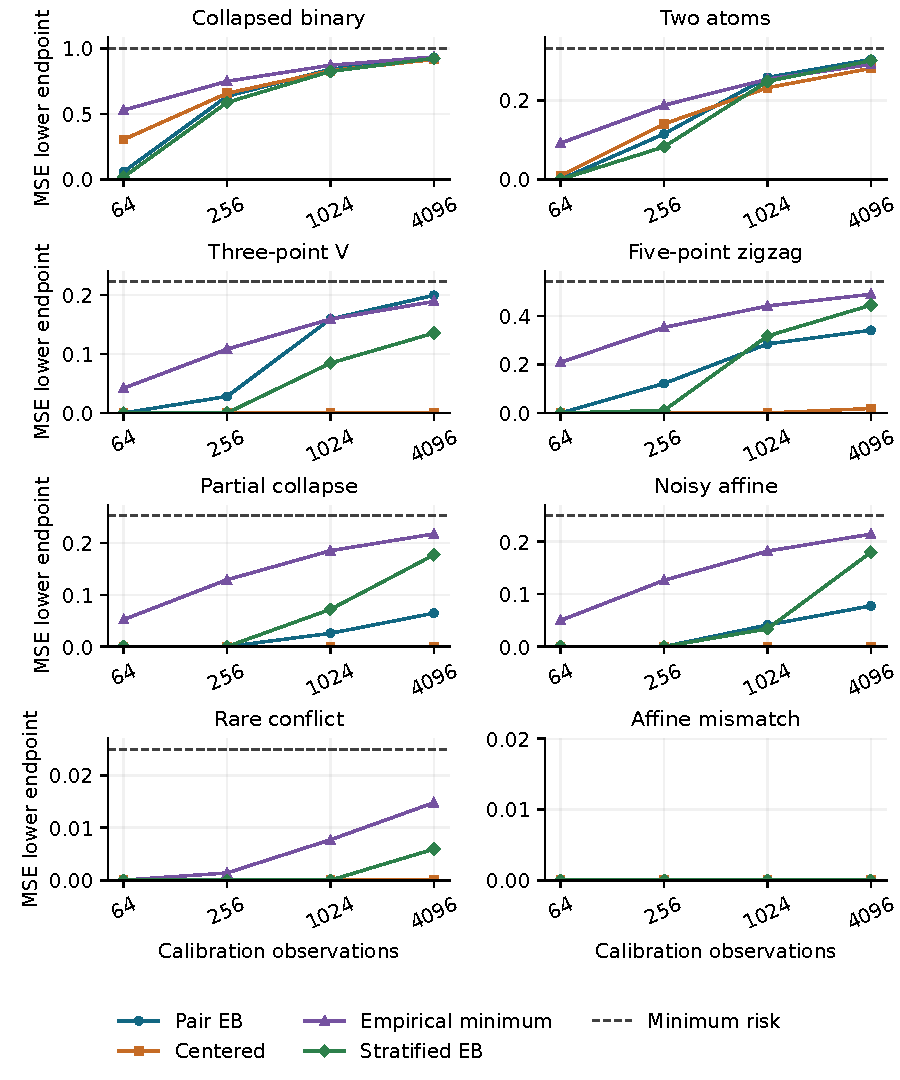
\includegraphics[width=\linewidth]{figures/witness_sample_size.pdf}
\caption{Mean lower endpoints over all 300 repetitions at each calibration
size for every prespecified law. Dashed lines show minimum population MSE.
Each method has its own $95\%$ one-sided confidence statement. Quantiles,
Monte Carlo uncertainty, secondary methods, and every trial are retained.}
\label{fig:witness-sample-size}
\end{figure}

\paragraph{Positive tolerances, coverage, and computation.}
The fixed RMSE tolerances are $0.10$, $0.25$, and $0.50$ for every law.
On partial collapse at $n=4096$, unconditional pairing excludes tolerance
$0.25$ in 211 of 300 trials; empirical minimization and primary stratification
both exclude it in all 300. Rare conflicts remain difficult: their exact
risk is $0.025$, but unconditional pairing and primary stratification never
exclude tolerance $0.10$ at this sample size. Empirical minimization excludes
it in all 300 trials. Tightening the stratified score range using the known
support raises its exclusion count to 284; additionally supplying known masses
raises it to 300. The gain therefore depends on both pairing and available
information.

All four primary methods have zero observed coverage violations across the
prespecified grid. This simulation does not prove coverage; each law--size
cell has only 300 repetitions, and the release gives binomial Monte Carlo
intervals. Reconstruction of all 76,800 primary and secondary endpoints
agrees within $1.12\times10^{-16}$. At $n=4096$, medians across the eight
law-wise median computation times are $31.3$, $34.7$, $265.4$, and $165.0$
$\mu$s for pair EB, centered, empirical minimum, and stratified EB,
respectively. These single-machine measurements use a precomputed finite-support
pair-score table and include sample statistics, confidence corrections, and
ERM optimization after representation lookup. They exclude feature learning
and do not establish a computational advantage on large continuous supports.
The frozen protocol, sufficient statistics, dual certificates, and complete
analysis are in \path{results/witness_comparison}.

\section{An analytic check of decision value}
\label{sec:decision-value}

An earlier controlled experiment uses explicit features to isolate the role
of lower calibration; its dictionaries are not learned KAHMs. Independent
episodes have history $X=(Z,S)$ and future
$Y=0.8SZ+0.1N$ (repairable) or $Y=0.8SR+0.1N$ (irreducible), where
$S\sim\operatorname{Bernoulli}(0.2)$ and $Z,R,N$ are independent random
signs. The retained blocks $(1)$, $(1-S,S)$, and
$((1+SZ)/2,(1-SZ)/2)$ have cumulative costs $1,3,5$ under budget
$\kappa=2$. Their exact minimum MSEs are $0.138,0.138,0.01$ in the
repairable regime and all $0.138$ in the irreducible regime. The fixed RMSE
tolerance $0.30$ therefore requires the last class in one regime and is
unattainable in the other. At cost 3, conditional pairing on $S$ raises
the population witness from $0.0324$ to $0.138$.

Each of 100 repetitions per regime uses 2048 training and 1024 validation
episodes, then calibration prefixes of $256,1024,4096,16384,65536$.
All decoders and the history partitions $S$ and $(S,Z)$ are frozen before
calibration. A $0.05$ failure budget covers all prefixes, sample sizes,
upper endpoints, and unconditional and stratified lower endpoints within
that regime--repetition.

Upper calibration accepts the repaired cost-5 predictor in all repetitions
from $n=1024$. Stratified lower calibration excludes both cheaper classes
in all repetitions at $n=16384$ and $65536$, certifying cost 5.
Unconditional lower calibration never closes the cost interval. Both rules
select the same predictor; lower evidence establishes the additional
class-level conclusion.

The irreducible control has no upper acceptance. Stratification excludes all
classes in 1 of 100 repetitions at $n=16384$ and all 100 at $65536$;
unconditional calibration never does. At $n=4096$, unconditional pairing
excludes the constant class in every repetition, while stratification excludes
none. All 600 fits converge, and all 200 observed simultaneous interval events
contain the exact risks. These results expose substantial sample requirements
and do not establish decision frequency in natural tasks. Complete details,
including all smaller-sample failures, remain in the source supplement
\path{sections/archive/decision_value_detailed.tex} and its associated tables
and figure.

\section{KAHM forecasting on bounded synthetic systems}
\label{sec:experiments}

The preceding studies test the general certificates. We now apply the
retained-dictionary learner to forecasting. All completed configurations and
unfavorable outcomes are retained. MSE denotes mean squared error and RMSE
its square root; empirical test error and a certified risk endpoint have
different interpretations.

\subsection{Protocol and predictive accuracy}

Four generators produce independent length-72 episodes: a noisy harmonic
oscillator, a quasiperiodic signal, nonlinear autoregression with bounded
innovations, and a logistic map with an episode-specific parameter. Their
observations lie in $[-1,1]$ by construction
(Appendix~\ref{app:protocols}). Each of five fitting repetitions uses 128
training, 512 validation, 4096 calibration, and 2048 test episodes. Histories
have lengths $m\in\{4,12\}$, horizons are $\{1,4,12\}$, and the 13 common
zero-based origins are $11,15,\ldots,59$. Within-episode windows may be
dependent. Geometry is relearned in each repetition, with budget $\kappa=4$,
ridge coefficient $10^{-4}$, affinity exponent $16$, and prefix dimensions
$2,6,14,30$. Geometry fitting uses at most 1600 histories and 24 local points.

Each repetition freezes 40 candidates: retained KAHM, RBF, and affine-hull
features; hard KAHM assignments; ordinary Frobenius-budget and exact-duplicate
ablations; ridge autoregression (AR); quadratic regression; KAHM and polynomial
feature rollouts; persistence; and a constant model. One candidate per family
is selected by validation MSE across horizons. These specified configurations
assess the procedure, rather than the best possible tuning of each family.

The failure budget $0.05$ per repetition allocates $0.04$ across
$2\times40\times3$ one-sided risk bounds and $0.01$ across 18 adjacent-prefix
improvement comparisons. Upper bounds use 4096 episode losses; lower bounds
use 2048 disjoint episode pairs. The 13 origins do not increase these independent
sample sizes. The joint event is per complete repetition, not across all runs.

\begin{table}[t]
\centering\small
\setlength{\tabcolsep}{4pt}
\begin{tabular}{lrrrrrrrr}
\toprule
& \multicolumn{2}{c}{Harmonic} & \multicolumn{2}{c}{Quasiperiodic} & \multicolumn{2}{c}{Nonlinear AR} & \multicolumn{2}{c}{Logistic}\\
Method & $h=1$ & $h=12$ & $h=1$ & $h=12$ & $h=1$ & $h=12$ & $h=1$ & $h=12$\\
\midrule
KAHM blocks & 0.070 & 0.346 & 0.078 & 0.284 & 0.054 & 0.074 & 0.176 & 0.511\\
RBF blocks & 0.068 & 0.351 & 0.068 & 0.287 & 0.057 & 0.074 & 0.172 & 0.512\\
Affine-hull blocks & 0.072 & 0.357 & 0.110 & 0.275 & 0.059 & 0.074 & 0.156 & 0.509\\
Hard KAHM states & 0.097 & 0.358 & 0.127 & 0.300 & 0.062 & 0.074 & 0.235 & 0.512\\
Ridge AR & 0.038 & 0.281 & 0.033 & 0.259 & 0.047 & 0.080 & 0.409 & 0.507\\
Quadratic regression & 0.031 & 0.243 & 0.030 & 0.246 & 0.047 & 0.081 & 0.010 & 0.508\\
KAHM rollout & 0.070 & 0.358 & 0.079 & 0.319 & 0.055 & 0.074 & 0.174 & 0.524\\
Polynomial rollout & 0.030 & 0.297 & 0.030 & 0.288 & 0.047 & 0.084 & 0.010 & 0.502\\
Persistence & 0.125 & 1.085 & 0.084 & 0.743 & 0.055 & 0.103 & 0.931 & 0.661\\
\bottomrule
\end{tabular}
\caption{Independent-test RMSE, averaged over five complete fitting seeds. One candidate per family is selected using development validation error averaged over all three horizons, before calibration or test scoring. The full archive includes $h=4$, seed variability, every candidate, and all confidence endpoints. These means are descriptive estimates, not population-risk certificates.}
\label{tab:forecast}
\end{table}


Table~\ref{tab:forecast} includes variation across the five fits. KAHM improves
substantially over long-horizon persistence on the periodic generators, but
quadratic and autoregressive models are stronger there. On nonlinear AR,
KAHM horizon-12 RMSE is $0.0743$, compared with $0.0802$ for ridge AR and
$0.0813$ for quadratic regression; the latter families are better at horizon
one. Direct KAHM fitting improves on feature rollout at horizon 12 on the two
periodic generators. The oscillator extension below gives counterexamples to
extending this ranking to every task.

\subsection{Acceptance, exclusion, and fitted refinement}

\begin{table}[t]
\centering\small
\begin{tabular}{lcccccc}
\toprule
& \multicolumn{3}{c}{KAHM retained family} & \multicolumn{3}{c}{All candidates}\\
System & $\epsilon=.20$ & $.35$ & $.50$ & $\epsilon=.20$ & $.35$ & $.50$\\
\midrule
Harmonic & 0/5 (--) & 0/5 (--) & 5/5 (6) & 0/5 (--) & 5/5 (12) & 5/5 (4)\\
Quasiperiodic & 0/5 (--) & 5/5 (14) & 5/5 (2) & 0/5 (--) & 5/5 (4) & 5/5 (1)\\
Nonlinear AR & 5/5 (2) & 5/5 (2) & 5/5 (2) & 5/5 (2) & 5/5 (2) & 5/5 (2)\\
Logistic & 0/5 (--) & 0/5 (--) & 0/5 (--) & 0/5 (--) & 0/5 (--) & 0/5 (--)\\
\bottomrule
\end{tabular}
\caption{Runs certifying the same RMSE tolerance at all horizons $1,4,12$. Parentheses give median retained feature dimension among successful least-dimension selections; `--' means no model passed. Cost is a representation-size proxy, not measured runtime. Each run has a joint 95\% event covering its complete frozen family and improvement comparisons.}
\label{tab:selection}
\end{table}


The retained KAHM family certifies the all-horizon RMSE requirement $0.20$
for every nonlinear-AR repetition, $0.35$ for every quasiperiodic repetition,
and $0.50$ for every harmonic repetition. Allowing all families also certifies
$0.35$ on harmonic data. No candidate certifies $0.50$ on the logistic task;
this is unresolved, not evidence that all true risks exceed the threshold.
Even the selected harmonic quadratic model's mean one-step test RMSE $0.0311$
corresponds to a mean upper endpoint $0.1497$, illustrating the precision cost.

Of 480 retained-KAHM candidate--horizon statements, 119 have positive lower
endpoints. Only two exclude RMSE $0.35$, and none excludes $0.50$; positive
endpoints alone are not enough for a useful positive-tolerance decision.
Section~\ref{sec:decision-value} reports the complete decision audit.
Paired comparisons certify 72 of 360 adjacent-prefix improvements. Nonlinear
AR has no certified adjacent-prefix gain despite meeting useful tolerances.
The complete refinement curves and system-specific counts are retained in
the repository; nesting a class does not guarantee improvement of each fit.

Exact duplication is already covered analytically by
Theorem~\ref{thm:replication-invariance}. Zero-ridge numerical checks reproduce
matching minimum training risks within their solver gaps. The main duplicate
candidate uses zero ridge, whereas primary models use $10^{-4}$; their fitted
errors are therefore not evidence for ridge-estimator invariance.
All 800 main-study candidates completed with recorded block-solver gaps below
$10^{-7}$. The original independent score audit reproduced all 4800 one-sided
endpoints and 360 improvement bounds exactly; a fresh harmonic replay also
matched 983,040 saved score entries. These numerical checks complement, rather
than replace, the probability arguments.

\paragraph{Earlier two-atom calibration.}
The original benchmark retains all 28,800 trials with analytically known class
and fitted risks (Appendix~\ref{app:known-risk}). One pair lower endpoint
exceeds its true risk; no centered lower or fitted upper endpoint does.
Its centered implementation added uncertainty to a known zero representation
variance. At full collapse and $n=4096$, its mean lower endpoint $0.5327$
therefore understates what a range-aware comparator can achieve: using the
known zero variance with the same target correction gives an expected endpoint
at least $0.9031$, versus the original pair mean $0.9177$.
The $n^{-1/4}$ penalty in that implementation is not intrinsic to centered
methods. The stronger comparisons in Section~\ref{sec:witness-comparison}
use direct standard-deviation concentration and a certified empirical minimum.

\subsection{Independently initialized Van der Pol and Duffing episodes}
\label{sec:oscillators}

To connect the learning experiment to the nonlinear oscillator setting of
\citet{kumar2026limits}, we apply the same frozen learning and certification
procedure to independently initialized Van der Pol and forced Duffing
episodes. The physical dynamics are
\begin{align*}
 \dot x&=v,&
 \dot v&=(1-x^2)v-x
 &&\text{(Van der Pol)},\\
 \dot x&=v,&
 \dot v&=-0.2v+x-x^3+0.3\cos(1.2t+\varphi)
 &&\text{(Duffing)}.
\end{align*}
Initial position and velocity are independently uniform on $[-2,2]$;
the Duffing forcing phase is uniform on $[0,2\pi]$ independently in each
episode. We integrate with classical fourth-order Runge--Kutta, step
$0.025$, discard ten time units, and sample 72 observations at interval
$0.1$. The forecast target is the explicitly defined noisy sensor
\[
 Y_j=0.95\tanh(x(10+0.1j))+\eta_j,\qquad
 \eta_j\stackrel{\mathrm{iid}}{\sim}\operatorname{Unif}[-0.02,0.02].
\]
This sensor has known range inside $[-0.97,0.97]$; the certificates use
the conservative range $[-1,1]$. Their units are sensor-output units.
They do not certify the error of an unobserved position or velocity estimate.
No stationarity or independence of windows within an episode is required.

Each system has three new complete fitting repetitions, with the same
128/512/4096/2048 training/validation/calibration/test episode counts,
histories, 40-candidate family, norm budget, and per-repetition joint
confidence allocation as the main experiment. Horizons $1,4,12$ correspond
to $0.1,0.4,1.2$ time units. The oscillator harness explicitly supplies the
generator to the unchanged main forecasting runner; its source hash and
all imported implementation hashes are retained. Within each method family,
the reported candidate minimizes development validation MSE averaged over
the horizons, before calibration or test evaluation. Every fitted candidate
and its episode scores are retained.

A numerical consistency check was specified before these runs. Sixteen
fixed initializations and their identical phases and observation noise were
integrated at steps $0.025$ and $0.0125$. The maximum sensor differences were
$1.69\times10^{-6}$ for Van der Pol and $3.49\times10^{-6}$ for Duffing,
both below the fixed $10^{-3}$ threshold. This is a half-step consistency
check of the numerical sampling law, rather than a rigorous global
continuous-time integration-error certificate.

\begin{table}[t]
\centering\small
\setlength{\tabcolsep}{3pt}
% Generated by experiments/run_oscillators.py; no manually entered results.
\begin{tabular}{llrrrr}
\toprule
System & Family & $h=1$ & $h=4$ & $h=12$ & $\overline U_{12}^{1/2}$ \\
\midrule
Van der Pol & KAHM blocks & $0.099\pm0.001$ & $0.139\pm0.005$ & $0.381\pm0.023$ & 0.409 \\
Van der Pol & RBF blocks & $0.106\pm0.005$ & $0.152\pm0.011$ & $0.383\pm0.010$ & 0.412 \\
Van der Pol & Affine blocks & $0.137\pm0.003$ & $0.192\pm0.006$ & $0.299\pm0.009$ & 0.333 \\
Van der Pol & Ridge AR & $0.038\pm0.000$ & $0.150\pm0.001$ & $0.353\pm0.001$ & 0.383 \\
Van der Pol & Quadratic direct & $0.032\pm0.000$ & $0.138\pm0.001$ & $0.342\pm0.001$ & 0.374 \\
Van der Pol & KAHM rollout & $0.034\pm0.012$ & $0.064\pm0.030$ & $0.341\pm0.033$ & 0.374 \\
Van der Pol & Quadratic rollout & $0.029\pm0.000$ & $0.127\pm0.002$ & $0.399\pm0.006$ & 0.427 \\
Van der Pol & Persistence & $0.089\pm0.000$ & $0.339\pm0.000$ & $0.868\pm0.001$ & 0.885 \\
Duffing & KAHM blocks & $0.080\pm0.002$ & $0.120\pm0.004$ & $0.250\pm0.010$ & 0.300 \\
Duffing & RBF blocks & $0.061\pm0.001$ & $0.098\pm0.003$ & $0.229\pm0.007$ & 0.281 \\
Duffing & Affine blocks & $0.064\pm0.004$ & $0.097\pm0.003$ & $0.223\pm0.005$ & 0.274 \\
Duffing & Ridge AR & $0.019\pm0.000$ & $0.041\pm0.000$ & $0.151\pm0.001$ & 0.214 \\
Duffing & Quadratic direct & $0.017\pm0.000$ & $0.035\pm0.000$ & $0.137\pm0.001$ & 0.203 \\
Duffing & KAHM rollout & $0.081\pm0.001$ & $0.126\pm0.004$ & $0.269\pm0.014$ & 0.315 \\
Duffing & Quadratic rollout & $0.017\pm0.000$ & $0.035\pm0.000$ & $0.140\pm0.002$ & 0.206 \\
Duffing & Persistence & $0.033\pm0.001$ & $0.114\pm0.002$ & $0.318\pm0.005$ & 0.363 \\
\bottomrule
\end{tabular}

\caption{Independent-test sensor RMSE, mean $\pm$ sample standard deviation
over three complete fitting repetitions. Each family is selected using
development validation data. The last column averages the corresponding
horizon-12 upper RMSE endpoints, namely
$3^{-1}\sum_{r=1}^3\sqrt{U_{r,12}}$; it is a descriptive summary of
individual certificates, not a newly calibrated ensemble guarantee.
All individual certificates and all 40 candidates per repetition are archived.}
\label{tab:oscillators}
\end{table}

Table~\ref{tab:oscillators} shows substantial long-horizon improvement over
persistence for the retained KAHM models: mean horizon-12 RMSE is $0.3814$
versus $0.8677$ on Van der Pol and $0.2499$ versus $0.3185$ on Duffing.
The comparison also exposes method-dependent limitations. The local
affine-hull blocks achieve $0.2990$ on Van der Pol, and direct quadratic
regression achieves $0.1369$ on Duffing. An iterated KAHM model has lower
mean horizon-12 error than direct KAHM fitting on Van der Pol
($0.3408$ versus $0.3814$), while direct fitting performs better in this
comparison on Duffing ($0.2499$ versus $0.2686$). Consequently, the earlier
advantage of direct fitting on the periodic generators should not be
extrapolated to all nonlinear oscillators.

The retained KAHM family certifies the all-horizon RMSE requirement $0.35$
in all three Duffing repetitions. For Van der Pol, it certifies $0.50$ in
all three repetitions but does not certify $0.35$. When all comparison
families are eligible, the $0.35$ requirement is certified in every
repetition of both systems. No candidate certifies the all-horizon
$0.20$ requirement in this follow-up. Adjacent KAHM refinements have
strictly positive certified improvement in 43 of 54 Van der Pol comparisons
and ten of 54 Duffing comparisons, using the same per-repetition multiplicity
allocation as before. These decisions distinguish an adequate fitted
model, an informative refinement, and an unresolved accuracy requirement.

All six scheduled runs completed, retaining 240 fitted candidates.
The independent score audit reconstructs their 1440 one-sided risk endpoints
and 108 paired improvement statements with zero numerical discrepancy.
The probability guarantees apply to the specified bounded sensor and the
fixed independent-episode numerical law; they do not transfer directly to
raw-state errors reported under a different observation protocol.

\subsection{Sensitivity to the coefficient budget}
\label{sec:budget-sensitivity}

The coefficient budget $\kappa$ defines the prediction class; its numerical
value is not directly comparable across feature maps. An unfavorable result
at one budget does not establish impossibility at larger budgets. This
follow-up was designed after inspecting the main results and uses new
development, calibration, and test random streams.

We fix $m=12$ and compare $\kappa\in\{1,4,16\}$ on all four main systems
with new seeds 2701--2703. Other settings are unchanged, including 128 training,
512 validation, 4,096 calibration, and 2,048 test episodes per repetition.
Each budget has 21 frozen candidates. Within each system and seed, budgets
share data streams and geometric blocks; only the coefficient constraint
changes. The study comprises 36 runs and 756 models.

For each system, seed, and budget, we select the retained KAHM prefix by mean
validation MSE over the three horizons. No budget is selected using test error.
We allocate failure probability $0.05/3$ to each budget's complete family of
risk bounds and paired comparisons. A union bound gives joint confidence at
least 0.95 across the three budgets within each system--seed repetition.
This event does not extend jointly across all twelve system--seed repetitions.
Table~\ref{tab:budget} reports test errors and all-horizon certification
counts at tolerance 0.35 for the validation-selected predictors.

\begin{table}[t]
  \centering
  \small
  \setlength{\tabcolsep}{4pt}
  % Automatically generated by experiments/run_sensitivity.py.
\begin{tabular}{llrrrrr}
\toprule
System & $\kappa$ & Features & $h=1$ & $h=4$ & $h=12$ & Passes \\
\midrule
Harmonic & 1 & 16.7 & 0.3737 & 0.4102 & 0.4696 & 0/3 \\
Harmonic & 4 & 30.0 & 0.1414 & 0.2313 & 0.3900 & 0/3 \\
Harmonic & 16 & 30.0 & 0.1392 & 0.2292 & 0.3875 & 0/3 \\
\addlinespace[2pt]
Quasiperiodic & 1 & 24.7 & 0.2510 & 0.2905 & 0.3336 & 0/3 \\
Quasiperiodic & 4 & 30.0 & 0.1294 & 0.2050 & 0.2927 & 3/3 \\
Quasiperiodic & 16 & 30.0 & 0.1294 & 0.2050 & 0.2927 & 3/3 \\
\addlinespace[2pt]
Nonlinear AR & 1 & 7.3 & 0.1059 & 0.1056 & 0.1068 & 3/3 \\
Nonlinear AR & 4 & 30.0 & 0.0670 & 0.0730 & 0.0746 & 3/3 \\
Nonlinear AR & 16 & 30.0 & 0.0670 & 0.0730 & 0.0746 & 3/3 \\
\addlinespace[2pt]
Logistic & 1 & 30.0 & 0.4713 & 0.5003 & 0.5052 & 0/3 \\
Logistic & 4 & 30.0 & 0.4384 & 0.4967 & 0.5044 & 0/3 \\
Logistic & 16 & 30.0 & 0.4384 & 0.4968 & 0.5044 & 0/3 \\
\bottomrule
\end{tabular}

  \caption{Sensitivity to the coefficient budget. Test RMSE and retained
  feature count are means over three new fitting seeds. ``Passes'' counts
  validation-selected KAHM predictors certified at tolerance 0.35
  simultaneously for $h=1,4,12$. All outcomes are retained. The confidence
  allocation covers all three budget families within each system--seed
  repetition.}
  \label{tab:budget}
\end{table}

Increasing the budget from 1 to 4 materially improves fitted KAHM prediction.
On the harmonic system, mean one-step RMSE decreases from 0.3737 to 0.1414;
on the nonlinear autoregression, it decreases from 0.1059 to 0.0670. On the
quasiperiodic system, the number of validation-selected models certified at
tolerance 0.35 increases from zero to three out of three. Thus the budget affects accuracy and certification.

Increasing the budget from 4 to 16 produces much smaller changes. Harmonic
horizon-12 RMSE changes from 0.3900 to 0.3875, and none of those KAHM models
passes the all-horizon 0.35 criterion. Quasiperiodic and nonlinear-AR results
are unchanged at the displayed precision. Logistic horizon-12 RMSE remains
approximately 0.5044, with no successful all-horizon certification. Thus increasing the budget alone to 16 leaves limitations in this
configuration, without establishing impossibility for richer geometries
or larger budgets.

The autoregressive and quadratic baselines fitted at the same numerical budgets
are retained in the released results. On the harmonic system at $\kappa=16$,
their mean horizon-12 RMSEs are 0.2377 and 0.2375, respectively, and both certify
all three repetitions at tolerance 0.35. On the nonlinear autoregression at
$\kappa=4$, KAHM has smaller horizon-12 RMSE (0.0746) than the autoregressive
(0.0800) and quadratic (0.0809) baselines, while its one-step error is larger.
These task- and horizon-specific comparisons retain the feature-dependent
capacity caveat above.

Every run retains its candidate descriptions, calibration losses, pair scores,
and test losses. An independent reconstruction audit passed for all 36 runs,
recomputing 2,268 candidate--horizon certificates and 324 paired improvement
bounds. All recorded constrained optimizations converged with reported gaps
below $10^{-7}$. The use of common random streams across budgets was also
verified. The checks support the numerical calculations and confidence allocation.

\subsection{Writer-disjoint forecasting of original pen trajectories}
\label{sec:pendigits}

We evaluate the same forecasters on original PenDigits trajectories
\citep{alpaydin1996pendigits}. Few writer groups are available, and the
risk theorem's independent-episode assumption is unverified.

\paragraph{Data and causal inputs.}
The University of California, Irvine (UCI) archive provides original
time-sampled pen locations and a table of eight spatially resampled locations
per digit. We use the original, unnormalized UNIPEN records because the
table's whole-character preprocessing is unsuitable for causal forecasting. The acquisition protocol specifies coordinates in $[0,500]^2$ and a
nominal sampling interval of $100$ ms. Each recorded coordinate $z$ is
transformed to $z/250-1$, and scalar predictions are clipped to $[-1,1]$.
We check every source coordinate against the declared acquisition range.
There is no per-stroke centering, alignment, normalization, or resampling.

The documented source split contains 7,494 digit records from 30 development
writers and 3,498 records from 14 different test writers. We infer writer
identity from the second integer in each UNIPEN \texttt{COMMENT} field: its
range and the approximately 250 records per identifier match the documented
writer counts. Because the source does not define these fields explicitly, writer identity
remains an inference. Identifiers include their source split. Pen-up gaps are
not treated as ordinary time steps.

We retain a digit's first pen-down stroke only if it contains at least 32
samples, and then use its first 32 points. This leaves 1,751 test digits from
13 eligible test writers; one of the original 14 writers has no qualifying
first stroke. The population is restricted to writers with eligible strokes. Eligibility
depends on completed stroke length, making this a retrospective task that
does not cover every newly started stroke. No loss
is assigned to the excluded writer. The eligible-writer count was corrected
from 14 to 13 before test scoring; the fixed eligibility rule was unchanged.
The released records document the correction.

\paragraph{Development and evaluation.}
Within the development file, the first 24 writer identifiers are used for
training and the remaining six for validation. Each of three fixed seeds
selects 20 eligible strokes per training writer, for 480 training strokes.
All 717 eligible strokes from the validation writers are used for selection.
The two coordinates are modeled separately, each from its own scalar history.
History lengths are $m\in\{4,8\}$, and forecast horizons are
$\mathcal H=\{1,2,4\}$ samples. The common zero-based forecast origins are
$7,11,15,19,23,27$. All models use causal histories and the same target origins.

For each coordinate and seed, the candidate family contains 40 models:
the three soft geometric feature families at four cumulative stages and two
history lengths; the KAHM ablations and feature-transition (Koopman) rollouts;
autoregressive and quadratic baselines; persistence; and a constant model.
Successive geometric block sizes are 2, 4, 8, and 16. Other settings are
$\kappa=4$, ridge coefficient $\lambda=10^{-4}$, and affinity exponent
$\omega=16$. We select one model per family by validation MSE, weighting
writers equally and averaging over the three horizons. All six
coordinate--seed families and their selections are frozen before test scoring.
Unselected candidates are also retained.

Within each writer, we average squared loss over origins and then eligible
digits. The cohort MSE gives each eligible writer equal weight. Let
$\widehat R_{c,r,h}$ denote this test MSE for coordinate $c\in\{1,2\}$,
fitting repetition $r\in\{1,2,3\}$, and horizon $h$. The coordinate-pooled
RMSE in a repetition is
\[
 \left(\frac{\widehat R_{1,r,h}+\widehat R_{2,r,h}}{2}\right)^{1/2}.
\]
Table~\ref{tab:pendigits} reports its mean and sample standard deviation over
the three development seeds. These deviations measure fitting variability on the same test cohort,
not uncertainty across independent cohorts. A normalized RMSE of 0.01
corresponds to 2.5 acquisition pixels.

\begin{table}[t]
  \centering
  \small
  \setlength{\tabcolsep}{3pt}
  % Automatically generated by experiments/run_pendigits.py; do not hand-edit numbers.
\begin{tabular}{lrrrr}
\toprule
Family & Features & $h=1$ & $h=2$ & $h=4$ \\
\midrule
KAHM blocks & 30.0 & $0.0466\pm0.0010$ & $0.0669\pm0.0013$ & $0.1127\pm0.0013$ \\
RBF blocks & 30.0 & $0.0421\pm0.0017$ & $0.0626\pm0.0019$ & $0.1105\pm0.0015$ \\
Affine-hull blocks & 30.0 & $0.0510\pm0.0152$ & $0.0664\pm0.0114$ & $0.1039\pm0.0053$ \\
KAHM, Frobenius budget & 30.0 & $0.0466\pm0.0010$ & $0.0669\pm0.0013$ & $0.1127\pm0.0013$ \\
KAHM duplicate blocks & 8.0 & $0.1386\pm0.0016$ & $0.1532\pm0.0018$ & $0.1822\pm0.0018$ \\
KAHM hard assignment & 16.0 & $0.0641\pm0.0004$ & $0.0856\pm0.0009$ & $0.1297\pm0.0014$ \\
KAHM Koopman rollout & 30.0 & $0.0473\pm0.0011$ & $0.0688\pm0.0018$ & $0.1177\pm0.0025$ \\
Ridge autoregression & 8.0 & $0.0130\pm0.0000$ & $0.0273\pm0.0000$ & $0.0679\pm0.0001$ \\
Quadratic regression & 14.0 & $0.0077\pm0.0000$ & $0.0178\pm0.0001$ & $0.0518\pm0.0001$ \\
Quadratic Koopman rollout & 14.0 & $0.0077\pm0.0000$ & $0.0185\pm0.0002$ & $0.0551\pm0.0005$ \\
Persistence & 4.0 & $0.0351\pm0.0000$ & $0.0696\pm0.0000$ & $0.1347\pm0.0000$ \\
Constant & 1.0 & $0.2207\pm0.0007$ & $0.2231\pm0.0007$ & $0.2273\pm0.0008$ \\
\bottomrule
\end{tabular}

  \caption{Original PenDigits forecasting on 1,751 eligible digits from 13
  held-out writers. Entries are coordinate-pooled RMSE, reported as mean
  $\pm$ sample standard deviation over three fitting seeds. ``Features'' is
  the mean retained feature count for the validation-selected models. Each
  scalar forecast uses only its own coordinate's history. All model selections
  precede test scoring.}
  \label{tab:pendigits}
\end{table}

\paragraph{Findings and limits.}
Quadratic regression is the most accurate reported family at all three
horizons. Its mean RMSEs are 0.00768, 0.01777, and 0.05184, compared with
0.04661, 0.06686, and 0.11269 for the KAHM block predictor. Ridge
autoregression also outperforms the KAHM block predictor. Relative to
persistence, KAHM is worse at one step and better at two and four steps.
These results do not establish general KAHM superiority. Retained-block
and ordinary Frobenius errors are effectively identical; the selected
retained-block norm sums are below $\kappa=4$, consistent with an inactive
constraint.

For completeness, we calculate upper bounds under an additional sampling
assumption: eligible writer records are iid from a common writer population
and independent of development records. The data documentation does not
establish this assumption. Each writer-averaged scalar loss lies in $[0,4]$.
Allocating total failure probability $0.05$ over two coordinates, three seeds,
40 candidates, and three horizons gives $2\cdot3\cdot40\cdot3=720$ one-sided
bounds. With 13 independent writers, the predeclared Hoeffding addition to
each empirical MSE is
\[
  4\sqrt{\frac{\log(720/0.05)}{2\cdot13}}=2.42741.
\]
Each resulting upper MSE bound is clipped at 4. Combining the two coordinate
bounds by the same averaging-and-square-root rule gives upper pooled-RMSE
endpoints of approximately 1.56, far above the observed errors and the
reported tolerances of 0.2, 0.35, and 0.5. None of these tolerances is certified.
The 1,751 trajectories and their overlapping prediction windows do not supply
1,751 independent writers. This experiment therefore provides descriptive
evidence about writer-disjoint forecasting and demonstrates the limited
usefulness of generic population certificates with few independent groups.

The release includes the official download URL and archive hash, parser,
length-filter accounting, training-record identifiers, frozen model descriptions,
and all 9,360 candidate--writer--horizon losses. Recomputing the cohort MSEs
from the exported losses agrees to within $1.4\times10^{-17}$. All recorded
block-norm budgets are feasible, and all reported optimization gaps are below
$10^{-7}$. These checks verify the reported numerical calculation; they do not
establish the iid-writer assumption.

\section{A follow-up comparison of KAHM input scaling}
\label{sec:input-scaling}

% Generated by scripts/make_scaling_assets.py; do not edit numeric cells.
\newcommand{\ScalingHarmonicOriginalMagnitude}{2.03}
\newcommand{\ScalingQuasiOriginalMagnitude}{2.32}
\newcommand{\ScalingNonlinearOriginalMagnitude}{0.18}
\newcommand{\ScalingLogisticOriginalMagnitude}{2.65}
\newcommand{\ScalingVDPOriginalMagnitude}{3.82}
\newcommand{\ScalingDuffingOriginalMagnitude}{7.07}
\newcommand{\ScalingPenOriginalMagnitude}{19.79}
\newcommand{\ScalingHardPenOriginalIncrease}{3.96}
\newcommand{\ScalingRolloutOriginalImprovingTasks}{7}
\newcommand{\ScalingHarmonicConfirmationMagnitude}{1.30}
\newcommand{\ScalingQuasiConfirmationMagnitude}{6.39}
\newcommand{\ScalingNonlinearConfirmationMagnitude}{1.31}
\newcommand{\ScalingLogisticConfirmationMagnitude}{6.97}
\newcommand{\ScalingVDPConfirmationMagnitude}{2.26}
\newcommand{\ScalingDuffingConfirmationMagnitude}{7.29}
\newcommand{\ScalingPenConfirmationMagnitude}{19.65}
\newcommand{\ScalingHardPenConfirmationIncrease}{4.14}
\newcommand{\ScalingRolloutConfirmationImprovingTasks}{6}
\newcommand{\ScalingRolloutVDPConfirmationMagnitude}{25.28}
\newcommand{\ScalingRolloutDuffingConfirmationMagnitude}{8.47}
\newcommand{\ScalingRolloutPenConfirmationMagnitude}{19.83}
\newcommand{\ScalingRolloutLogisticConfirmationMagnitude}{3.61}


The preceding experiments standardize history coordinates using their training
means and standard deviations. Although raw observations lie in $[-1,1]$,
standardized histories need not. We therefore test whether scaling training
histories to $[-1,1]$ benefits KAHMs, whose reconstruction regularization and
folding score depend on input magnitudes and geometry. Target bounds alone do
not specify KAHM input scale.

\subsection{A fixed intervention and two types of replication}

For coordinate $j$ of a history vector $x$, let $x_j$ denote its value, and let
$a_j$ and $b_j$ be the minimum and maximum over all training histories. These
extrema are computed before subsampling histories for geometry fitting. The
primary alternative to standardization is the min--max transformation
\begin{equation}
 z_j(x)=
 \begin{cases}
  2\dfrac{x_j-a_j}{b_j-a_j}-1,&b_j>a_j,\\[4pt]
  0,&b_j=a_j.
 \end{cases}
 \label{eq:input-minmax}
\end{equation}
Training extrema remain fixed for validation, calibration, and testing; none
are estimated from these data or a completed test trajectory. Unseen values
can map outside $[-1,1]$; this primary preprocessing variant, or \emph{arm},
does not clip them. A diagnostic arm applies
$\widetilde z_j(x)=\max\{-1,\min\{1,z_j(x)\}\}$, and another uses bounded raw
histories. Constant training coordinates map to zero in both min--max arms.
Together with standardization, these give four arms.

The intervention changes only the inputs to KAHM geometry and to models built
from it: retained-block, single-Frobenius-budget, duplicate-block,
hard-assignment, and feature-rollout models. The non-KAHM feature families,
forecast targets, output clipping, coefficient budgets, ridge coefficient,
affinity exponent, history lengths, origins, sample counts, local-point limits,
and random streams remain unchanged. Within each arm, each model family selects
its history length and dictionary stage by mean validation MSE across horizons.
Test error is not used to choose among preprocessing arms.

The first comparison pairs all four arms on identical data for every original
fitting seed and coefficient-budget condition. The scaling hypothesis followed
inspection of the original study, so these reused streams are not a new test
set. The primary outcome, alternatives, selection rule, and schedule were
recorded before examining the scaling results; all outcomes, including
regressions, are retained. The exact-risk two-atom experiment and analytic
duplicate-invariance illustration do not fit KAHM input geometry and therefore
admit no scaling intervention.

For confirmation, we fixed the same four arms and used fitting seeds
$4701$--$4703$ on all six synthetic systems. The original stream-offset rule
then generates new training, validation, calibration, and test episodes, with
the original sample counts and main-study budget $\kappa=4$. This adds 18
paired synthetic repetitions, without tuning between the replay and confirmation
stages. For PenDigits, the same three new seeds select new training subsamples
from the existing development writers. The validation writers and held-out
writer cohort remain unchanged. Thus the PenDigits confirmation assesses
variation across training subsamples on a fixed cohort, rather than variation
across newly sampled writers.

\subsection{Accuracy gains, regressions, and fitting variation}

% Generated by scripts/make_scaling_assets.py; do not edit numeric cells.
\begin{table}[tbp]
\centering\small
\setlength{\tabcolsep}{2.5pt}
\begin{tabular}{lrrrrrrrr}
\toprule
& \multicolumn{4}{c}{Original fitting seeds} & \multicolumn{4}{c}{New fitting seeds}\\
\cmidrule(lr){2-5}\cmidrule(lr){6-9}
Task & Standard & Min--max & $\Delta\%$ & Wins & Standard & Min--max & $\Delta\%$ & Wins\\
\midrule
Harmonic & 0.049148 & 0.048150 & -2.03 & 4/5 & 0.050240 & 0.049586 & -1.30 & 3/3\\
Quasiperiodic & 0.037040 & 0.036182 & -2.32 & 3/5 & 0.038290 & 0.035842 & -6.39 & 3/3\\
Nonlinear AR & 0.004561 & 0.004569 & +0.18 & 4/5 & 0.004718 & 0.004656 & -1.31 & 2/3\\
Logistic & 0.164577 & 0.168931 & +2.65 & 1/5 & 0.164632 & 0.176103 & +6.97 & 0/3\\
Van der Pol & 0.058343 & 0.060572 & +3.82 & 0/3 & 0.054809 & 0.056049 & +2.26 & 1/3\\
Duffing & 0.027776 & 0.025812 & -7.07 & 3/3 & 0.027913 & 0.025877 & -7.29 & 3/3\\
PenDigits & 0.006449 & 0.005173 & -19.79 & 3/3 & 0.006792 & 0.005457 & -19.65 & 3/3\\
\bottomrule
\end{tabular}
\caption{Validation-selected retained KAHM predictors: mean test MSE over all three horizons and fitting seeds. The primary alternative is training min--max scaling without query clipping. $\Delta\%=100(\mathrm{MSE}_{\rm minmax}/\mathrm{MSE}_{\rm standard}-1)$; negative values denote improvement. Wins counts fitting repetitions with a smaller all-horizon MSE. Original main tasks have five repetitions; original oscillators and PenDigits have three. All new-seed comparisons have three. Synthetic confirmation uses new development, calibration, and test episodes. PenDigits confirmation uses new training subsamples and the same held-out writer cohort, with coordinate MSE pooled before averaging horizons. Original-seed results reuse previously evaluated streams and are descriptive. No average across different task units is taken.}
\label{tab:input-scaling-primary}
\end{table}


Table~\ref{tab:input-scaling-primary} reports the primary comparison for all
tasks. Mean all-horizon MSE decreases on the harmonic, quasiperiodic, and
Duffing systems in both stages. The Duffing reduction is
\ScalingDuffingOriginalMagnitude\% on the original seeds and
\ScalingDuffingConfirmationMagnitude\% on the new seeds. The nonlinear
AR effect is small and changes sign between stages. Logistic error increases
by \ScalingLogisticOriginalMagnitude\% and
\ScalingLogisticConfirmationMagnitude\%, and Van der Pol error increases by
\ScalingVDPOriginalMagnitude\% and \ScalingVDPConfirmationMagnitude\%.
An improvement averaged over horizons need not hold at every horizon. For
example, on the original quasiperiodic repetitions, short-horizon gains
accompany an increase in horizon-12 mean RMSE from 0.2841 to 0.2894.

% Generated by scripts/make_scaling_assets.py; do not edit numeric cells.
\begin{table}[tbp]
\centering\small
\setlength{\tabcolsep}{4pt}
\begin{tabular}{lrrrr}
\toprule
& \multicolumn{2}{c}{Original fitting seeds} & \multicolumn{2}{c}{New fitting seeds}\\
\cmidrule(lr){2-3}\cmidrule(lr){4-5}
Task & $\overline\Delta\pm s_\Delta$ & $\mathrm{SE}_{\rm ep}$ & $\overline\Delta\pm s_\Delta$ & $\mathrm{SE}_{\rm ep}$\\
\midrule
Harmonic & $-0.9977\pm1.2991$ & 0.0360 & $-0.6544\pm0.1582$ & 0.0198\\
Quasiperiodic & $-0.8578\pm1.8211$ & 0.0488 & $-2.4482\pm1.3631$ & 0.0630\\
Nonlinear AR & $+0.0083\pm0.0786$ & 0.0089 & $-0.0619\pm0.0935$ & 0.0151\\
Logistic & $+4.3538\pm5.1613$ & 0.1365 & $+11.4711\pm6.6749$ & 0.2367\\
Van der Pol & $+2.2297\pm1.6634$ & 0.1242 & $+1.2396\pm4.2734$ & 0.1101\\
Duffing & $-1.9642\pm1.4355$ & 0.0950 & $-2.0360\pm0.3666$ & 0.0692\\
PenDigits & $-1.2760\pm0.4998$ & -- & $-1.3346\pm0.1942$ & --\\
\bottomrule
\end{tabular}
\caption{Two distinct sources of variation for the primary scaling comparison. All numbers are in units of $10^{-3}$ MSE for the corresponding task. $\Delta$ is min--max minus standard MSE after averaging horizons within a repetition; $s_\Delta$ is its sample SD across complete fitting repetitions. $\mathrm{SE}_{\rm ep}$ measures paired test-episode Monte Carlo uncertainty of the mean difference, conditional on the fitted, validation-selected models. It does not measure training variability. No iid-writer SE is assigned to the fixed PenDigits cohort. Original-seed quantities reuse previously evaluated streams and are descriptive. Neither column is a finite-sample certificate of an algorithm-level gain.}
\label{tab:input-scaling-uncertainty}
\end{table}


Table~\ref{tab:input-scaling-uncertainty} distinguishes complete fitting
repetitions from test episodes evaluating a fitted model. Let $\Delta$ be
min--max MSE minus standardized-input MSE per repetition, with mean
$\overline\Delta$ and sample standard deviation $s_\Delta$ across repetitions.
The standard error $\mathrm{SE}_{\rm ep}$ accounts for finitely many independent
test episodes, conditional on the fitted, validation-selected models. We
average paired loss differences over horizons within each episode, estimate
the variance of each repetition's mean difference, and combine these variances
for the mean across repetitions. Many episodes can yield a small conditional
standard error without providing many independent fits.

The mean MSE change can oppose the majority of seed-specific effects because
their magnitudes differ. Every seed's sign and effect size are archived.
Neither a small conditional standard error nor a favorable mean establishes
improvement for a newly fitted model.

% Generated by scripts/make_scaling_assets.py; do not edit numeric cells.
\begin{table}[tbp]
\centering\small
\setlength{\tabcolsep}{4pt}
\begin{tabular}{llrrr}
\toprule
Fitting seeds & Input preprocessing & $h=1$ & $h=2$ & $h=4$\\
\midrule
1701--1703 & Standardization & $0.04661\pm0.00098$ & $0.06686\pm0.00134$ & $0.11269\pm0.00132$\\
1701--1703 & Min--max & $0.03693\pm0.00228$ & $0.05667\pm0.00257$ & $0.10454\pm0.00300$\\
\midrule
4701--4703 & Standardization & $0.04816\pm0.00199$ & $0.06884\pm0.00223$ & $0.11536\pm0.00202$\\
4701--4703 & Min--max & $0.03950\pm0.00123$ & $0.05922\pm0.00128$ & $0.10631\pm0.00090$\\
\bottomrule
\end{tabular}
\caption{PenDigits retained KAHM forecasting: mean $\pm$ sample SD of coordinate-pooled RMSE over three fitting seeds. Coordinate MSE is pooled before taking each seed's square root. All 1,751 eligible digits and 13 held-out writers are identical across both seed sets and preprocessing arms. The SD measures fitting variation on this cohort, not uncertainty across independent test cohorts. A normalized error of 0.01 corresponds to 2.5 acquisition pixels.}
\label{tab:input-scaling-pendigits}
\end{table}


The retained soft KAHM predictor has its largest relative gain on PenDigits:
cohort MSE, averaged over coordinates and horizons, decreases by
\ScalingPenOriginalMagnitude\% in the replay and
\ScalingPenConfirmationMagnitude\% with the new training subsamples.
Table~\ref{tab:input-scaling-pendigits} reports horizon-specific RMSE and its
variation across fitting seeds. All three horizons improve for each coordinate
and each fitting seed in both stages. Every held-out writer also has a smaller
mean loss, averaged over coordinates and horizons, in each seed. These
comparisons repeatedly evaluate the same 13 writers and do not establish a
claim about a population of independently sampled writers. Quadratic
regression and ridge AR remain more accurate than the scaled retained KAHM
predictor on this task; its one-step error also remains above persistence.

The gain does not extend to every predictor built from KAHM features. On
PenDigits, the hard-assignment model's all-horizon MSE increases by
\ScalingHardPenOriginalIncrease\% on the original seeds and
\ScalingHardPenConfirmationIncrease\% on the new seeds, with degradation in
every fitting repetition. The complete records also retain the other KAHM
ablations and rollouts. These results support a scaling benefit for particular
soft representations under the stated protocol, rather than for all KAHM
models.

As a separate secondary outcome, KAHM feature rollout has smaller mean
all-horizon MSE on \ScalingRolloutOriginalImprovingTasks\ of seven original
tasks and \ScalingRolloutConfirmationImprovingTasks\ of seven new-seed tasks.
The new-seed reductions include \ScalingRolloutVDPConfirmationMagnitude\%
on Van der Pol, \ScalingRolloutDuffingConfirmationMagnitude\% on Duffing,
and \ScalingRolloutPenConfirmationMagnitude\% on PenDigits. Logistic rollout
instead worsens by \ScalingRolloutLogisticConfirmationMagnitude\%.

\subsection{Diagnostic arms, coefficient budgets, and certification}

% Generated by scripts/make_scaling_assets.py; do not edit numeric cells.
\begin{table}[tbp]
\centering\small
\setlength{\tabcolsep}{5pt}
\begin{tabular}{lrrrr}
\toprule
& \multicolumn{2}{c}{Original fitting seeds} & \multicolumn{2}{c}{New fitting seeds}\\
\cmidrule(lr){2-3}\cmidrule(lr){4-5}
Task & Clipped min--max & Raw histories & Clipped min--max & Raw histories\\
\midrule
Harmonic & -2.03 & -1.59 & -1.30 & -1.79\\
Quasiperiodic & -2.31 & -3.96 & -6.39 & -6.75\\
Nonlinear AR & +0.18 & -0.74 & -1.31 & -1.52\\
Logistic & +2.65 & +3.87 & +6.97 & +4.80\\
Van der Pol & +3.82 & +5.27 & +2.26 & +4.79\\
Duffing & -7.07 & -13.30 & -7.30 & -11.59\\
PenDigits & -19.78 & -18.51 & -19.64 & -14.57\\
\bottomrule
\end{tabular}
\caption{Diagnostic preprocessing arms, reported as percent change in all-horizon test MSE relative to standardization for the retained KAHM family. Negative values denote improvement. Clipped min--max fixes all query inputs inside $[-1,1]$; raw histories use the task's existing bounded observations without standardization. These test comparisons are descriptive and are not used to choose a preprocessing arm per task. New-seed PenDigits results use the same writer cohort.}
\label{tab:input-scaling-diagnostics}
\end{table}

% Generated by scripts/make_scaling_assets.py; do not edit numeric cells.
\begin{table}[tbp]
\centering\small
\setlength{\tabcolsep}{5pt}
\begin{tabular}{lrrrrrr}
\toprule
& \multicolumn{2}{c}{$\kappa=1$} & \multicolumn{2}{c}{$\kappa=4$} & \multicolumn{2}{c}{$\kappa=16$}\\
\cmidrule(lr){2-3}\cmidrule(lr){4-5}\cmidrule(lr){6-7}
Task & $\Delta\%$ & Wins & $\Delta\%$ & Wins & $\Delta\%$ & Wins\\
\midrule
Harmonic & +0.41 & 2/3 & +0.17 & 2/3 & -1.24 & 2/3\\
Quasiperiodic & -1.16 & 1/3 & -4.94 & 3/3 & -4.94 & 3/3\\
Nonlinear AR & +0.01 & 1/3 & -0.59 & 2/3 & -0.59 & 2/3\\
Logistic & -0.13 & 1/3 & +1.89 & 0/3 & +1.87 & 0/3\\
\bottomrule
\end{tabular}
\caption{Scaling comparison within the original coefficient-budget sensitivity protocol: history length 12, seeds 2701--2703, and the same data across budgets. Entries are the percent change in mean all-horizon test MSE for training min--max scaling relative to standardization, plus the number of improving fitting seeds. Every stage is selected by mean validation MSE within its arm and budget. Negative values denote improvement. This comparison reuses the original sensitivity streams and is reported separately from the fresh six-system confirmation.}
\label{tab:input-scaling-budget}
\end{table}


Clipped and unclipped min--max scaling give similar retained KAHM results;
raw histories can change accuracy differently
(Table~\ref{tab:input-scaling-diagnostics}). Both diagnostic arms retain the
logistic and Van der Pol limitations, so histories lying in $[-1,1]$ do not
ensure improvement. Raw histories remove centering and variance normalization;
min--max scaling changes location and coordinate scale. The study does not
isolate individual components of KAHM geometry.

Table~\ref{tab:input-scaling-budget} reports every original coefficient-budget
condition. At $\kappa=1$, the mean effects are small and the signs differ across
seeds. At $\kappa=4$ and 16, the quasiperiodic comparison improves in all three
repetitions, while the logistic comparison worsens in all three. The harmonic
mean change has different signs at different budgets. Neither the budget nor
the preprocessing arm is selected by test performance. These results limit
extrapolation of a gain from one coefficient class to another.

At RMSE tolerances $0.20$, $0.35$, and $0.50$, standardization and primary
min--max scaling give equal counts of repetitions whose retained KAHM upper
endpoints meet the requirement at every horizon, for every original synthetic
system and budget and every synthetic confirmation system. PenDigits retains
its small writer cohort and uninformative nominal endpoints. Failure
allocations cover multiplicity within each arm, but not selection across arms.
A confidence interpretation requires arm specification independent of
calibration outcomes. Fixing the replay protocol before rerunning previously
used streams does not establish this independence; replay endpoints are
nominal. Fresh synthetic confirmation episodes support the stated within-arm
guarantees. New PenDigits fitting seeds still reuse previously examined
writers. The cross-arm accuracy comparisons therefore do not certify
preprocessing improvements.

\paragraph{Reproducibility and interpretation.}
The standardization replay exactly reproduces all retained non-timing results.
Across arms, non-KAHM models retain identical numerical results and saved
synthetic score arrays; writer-level control losses are also unchanged.
Four truncated score archives---two
per stage---were regenerated with the same source, configuration, and seeds;
non-timing records and candidate descriptions agree exactly. Damaged and
regenerated file hashes and replay records are retained. Reporting followed
archive-integrity checks and independent aggregation of the selected models'
test scores.

Standardization remains the reference preprocessing for the original
experiments. The repeated PenDigits and Duffing gains, together with the
logistic and Van der Pol regressions, show that the benefit of input scaling
depends on the task and prediction architecture.

\section{A matched comparison of KAHM and alternative geometries}
\label{sec:matched-geometry}

% Generated from the complete matched-geometry analysis.
\newcommand{\MatchedCandidates}{13{,}440}
\newcommand{\MatchedComparisons}{42}
\newcommand{\MatchedImproved}{28}
\newcommand{\MatchedDegraded}{14}
\newcommand{\MatchedCalComparisons}{180}
\newcommand{\MatchedCalCertified}{1}


The preceding experiments do not fully separate geometry and decoder effects:
the KAHM Frobenius-budget and rollout families lack corresponding radial basis
function (RBF) and affine-hull controls. We compare all three geometries with
identical decoder choices and validation opportunities on all seven tasks.
The protocol was specified before fitting, informed by the earlier experiments.

\subsection{Design and validation selection}

Each geometry is paired with three prediction architectures, referred to as
\emph{heads} in the tables. \emph{Block direct} predicts the requested horizons
under the sum-of-block-Frobenius-norms constraint in
\eqref{eq:training-objective}. \emph{Frobenius direct} uses a single Frobenius
norm constraint on the concatenated coefficient matrix. \emph{Rollout} fits an
affine transition between feature vectors, iterates this transition, and
decodes the resulting vector into the observed signal
(Appendix~\ref{app:protocols}). Every geometry--head pair has access to the four
retained dimensions $2,6,14,30$, both history lengths, and all four preprocessing
options from Section~\ref{sec:input-scaling}. Unlike the preceding scaling
study, this comparison varies preprocessing for KAHM, RBF, and affine-hull
features alike.

Training data, horizons, origins, regularization, geometry subsampling, and
target units follow the original configurations. Direct heads share a numerical
coefficient budget, which does not make feature maps statistically equivalent.
Rollout sensitivity budgets use the fitted transition and output decoder.
Equal feature counts need not imply equal runtime or kernel-evaluation cost.

The five fitting seeds $5701$--$5705$ generate new training, validation,
calibration, and test episodes for every synthetic task. PenDigits uses new
training-stroke subsamples and geometry-fitting randomness within the same
development and held-out writer cohorts, measuring fitting variation without
new test writers.

For each task, seed, geometry, and head, the primary analysis selects
preprocessing, history length, and retained dimension by mean validation MSE
across horizons. Ties are resolved by feature count, history length,
preprocessing order (standardization, min--max, clipped min--max, raw), and
candidate name. This gives six primary comparisons per task and seed: KAHM
against each of the two alternative geometries under each of the three heads.
The selected dimension, history, and preprocessing can differ between
geometries, but the available choices are identical.

The descriptive outcome is test MSE averaged over horizons; percentage changes
use ratios of seed-averaged MSEs, not means of seed-specific percentages. Every
paired seed effect is retained; tasks are not pooled. Additional curves fix
the dimension and select history length and preprocessing by validation.
A secondary analysis also selects the head by validation; it appears in
\path{taskwise_comparisons.csv}, in rows marked
\texttt{analysis=head\_selected} and \texttt{horizon=all};
Appendix~\ref{app:matched-geometry} gives the analysis directory.

PenDigits selects each coordinate's predictor separately and weights validation
writers equally. After selection, coordinate losses and horizon losses are
averaged within each held-out writer, and the 13 writers receive equal weight.
Repeated fitting seeds do not provide additional independent writers.

\subsection{Confidence accounting and interpretation}

For each synthetic task and seed, each arm receives failure budget $0.01$:
the inherited $80/20$ allocation assigns $0.008$ to fixed candidate risk bounds
and $0.002$ to refinement comparisons. A union bound over four arms uses $0.04$;
the remaining $0.01$ is divided equally among the six primary geometry
comparisons.

For each primary comparison, we subtract KAHM squared loss from the
alternative's squared loss and average the difference over horizons within
each independent calibration episode. The resulting episode averages lie in
$[-4,4]$. Applying the paired empirical Bernstein bound
\eqref{eq:paired-improvement}, with range length $8$ and failure probability
$0.01/6$, gives a lower confidence bound on the alternative's risk minus KAHM's
risk. A positive lower endpoint certifies lower risk for that fitted KAHM
predictor. All validation selection occurs before calibration and uses
independent development data.

This allocation gives a simultaneous $95\%$ event within each synthetic
task--seed combination, not across tasks, seeds, or earlier campaigns.
Fixed-dimension and head-selected comparisons remain descriptive; an
inconclusive improvement certificate does not establish equal risks.

PenDigits retains nominal writer-level upper endpoints with failure budget
$0.0125$ per
preprocessing arm, allocated jointly over candidates, coordinates, fitting
seeds, and horizons. The allocations sum to
$0.05$. A joint confidence interpretation requires both independent and
identically distributed writers and candidate specification independent of
the writer losses used for calibration. The first assumption remains unverified;
the second is not established for this follow-up because the design was
informed by earlier results on the same cohort. Consequently, these endpoints
do not provide a new confirmatory population guarantee. No additional
independent writer cohort is available for the geometry comparisons, and
paired writer differences remain descriptive.

\subsection{Geometry, prediction architecture, and task interact}

\begin{table}[t]
\centering
\small
\setlength{\tabcolsep}{3.5pt}
\begin{tabular}{lrrrrrr}
\toprule
& \multicolumn{2}{c}{Block direct} & \multicolumn{2}{c}{Frobenius direct} & \multicolumn{2}{c}{Rollout} \\
\cmidrule(lr){2-3}\cmidrule(lr){4-5}\cmidrule(lr){6-7}
Task & RBF & Affine & RBF & Affine & RBF & Affine \\
\midrule
Harmonic & $-2.4$ (5) & $-5.1$ (5) & $-1.5$ (5) & $+6.1$ (0) & $-0.2$ (3) & $+1.2$ (1) \\
Quasiperiodic & $-2.0$ (2) & $-1.4$ (2) & $-1.7$ (3) & $+30.1$ (0) & $-6.1$ (2) & $+3.3$ (1) \\
Nonlinear AR & $-2.7$ (5) & $-4.4$ (5) & $-2.7$ (5) & $-4.4$ (5) & $-5.0$ (5) & $-4.9$ (5) \\
Logistic & $-1.0$ (3) & $-4.5$ (5) & $-0.4$ (2) & $-5.8$ (5) & $+1.7$ (1) & $-5.7$ (5) \\
Van der Pol & $-14.4$ (5) & $+9.5$ (2) & $-14.5$ (3) & $+102.7$ (0) & $-17.1$ (4) & $+92.8$ (0) \\
Duffing & $+3.8$ (3) & $+13.1$ (1) & $+10.4$ (0) & $+70.6$ (0) & $+1.4$ (3) & $+79.9$ (0) \\
PenDigits & $-15.6$ (5) & $-12.7$ (4) & $-17.2$ (5) & $-1.9$ (4) & $-17.9$ (5) & $-1.4$ (3) \\
\bottomrule
\end{tabular}
\caption{Matched geometry follow-up: percentage change in test MSE of KAHM relative to the indicated alternative, within each head. Negative values favor KAHM. Parentheses give the number of 5 fitting seeds with lower KAHM MSE. Preprocessing, history and retained dimension are selected separately for each geometry and head by validation MSE only. Percentages use ratios of MSE averaged over horizons and fitting seeds within each task; PenDigits first pools coordinate losses and equally weights eligible writers. Synthetic calibration comparisons use new episodes and a separate multiplicity allocation. The PenDigits comparisons reuse the same cohort. All test effects in this table are descriptive.}
\label{tab:matched-geometry-primary}
\end{table}


All scheduled fits completed, yielding \MatchedCandidates\ retained candidates.
Table~\ref{tab:matched-geometry-primary} reports all \MatchedComparisons\ primary
task--head--alternative contrasts: KAHM has lower mean test MSE in
\MatchedImproved\ and higher mean test MSE in \MatchedDegraded. These contrasts
share tasks and fitted models; they are not independent evidence for a
universally preferred geometry. Table~\ref{tab:matched-geometry-mse} gives
absolute errors for all nine geometry--head families.

On nonlinear AR, KAHM improves on both geometric alternatives under every head
in all five fitting seeds. Its block-direct mean MSE is $0.00456$, compared
with $0.00511$ for ridge AR and $0.00523$ for quadratic regression. On PenDigits,
the KAHM reductions relative to RBF are $15.6\%$, $17.2\%$, and $17.9\%$ for
block direct, Frobenius direct, and rollout, respectively, with lower loss in
all five seeds. The corresponding mean reductions relative to affine-hull
features are $12.7\%$, $1.9\%$, and $1.4\%$, with four, four, and three favorable
seeds. This advantage is specific to the geometric comparison. PenDigits
Frobenius-direct KAHM MSE is $0.00504$, while ridge AR and quadratic regression
achieve smaller MSEs of $0.00184$ and $0.00102$.

The oscillator controls limit how much of an accuracy gain can be attributed
to KAHM geometry. On Van der Pol, KAHM mean MSE is $14.4$--$17.1\%$ lower than
RBF across the three heads, yet exceeds affine-hull MSE by $9.5\%$, $102.7\%$,
and $92.8\%$, respectively. On Duffing, the corresponding excesses over
affine-hull MSE are $13.1\%$, $70.6\%$, and $79.9\%$. The affine-hull advantage
under Frobenius-direct and rollout heads occurs in every fitting seed on both
oscillators. A gain from changing a KAHM decoder or its preprocessing therefore
does not by itself establish a benefit of KAHM geometry. Mean effects can also
disagree with most seed-specific effects: the favorable quasiperiodic
block-direct means against both alternatives occur with lower KAHM loss in
only two of five seeds.

\begin{figure}[p]
\centering
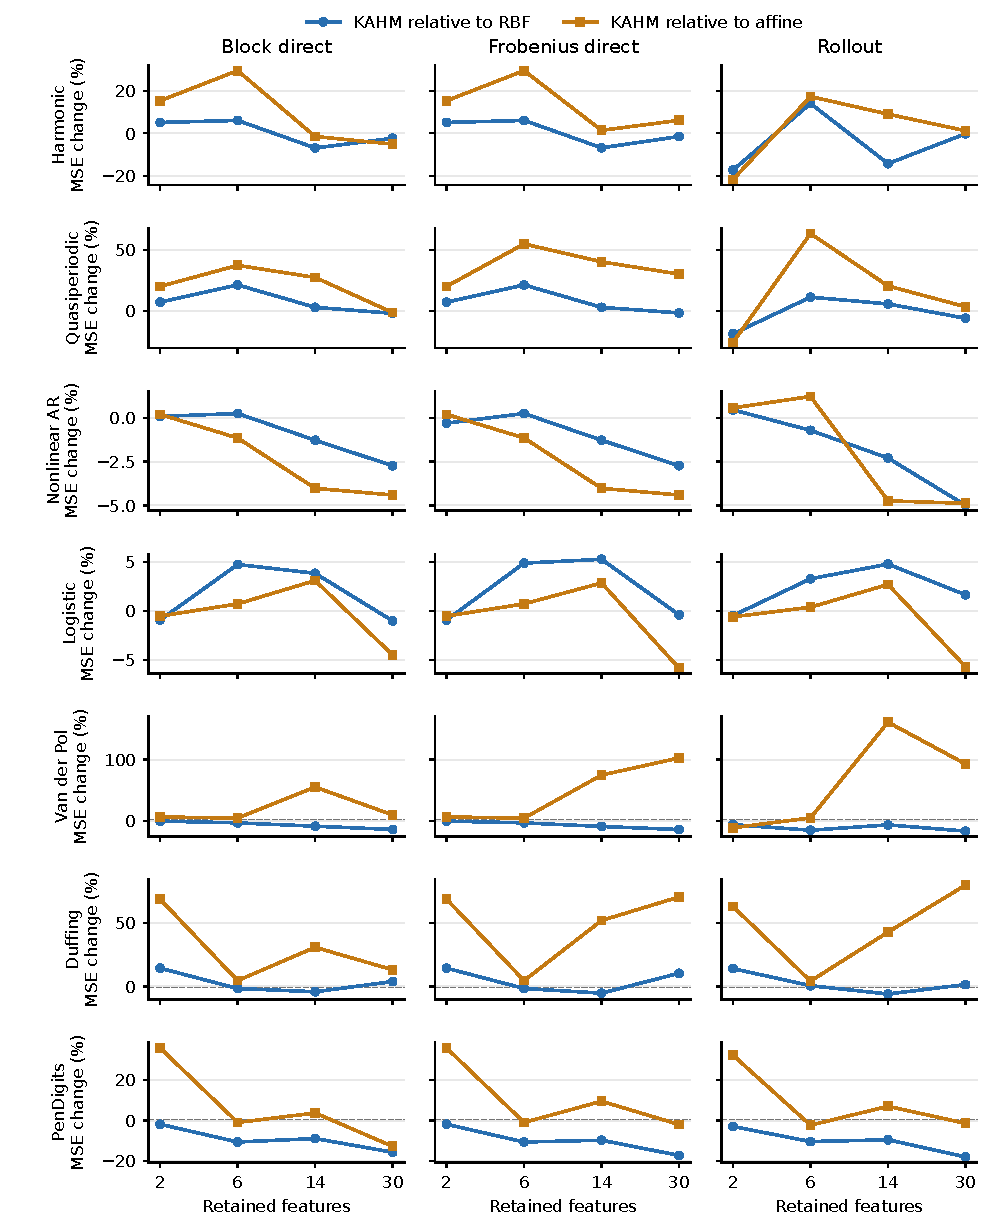
\includegraphics[width=\linewidth]{figures/matched_geometry_dimensions.pdf}
\caption{Percentage change in mean all-horizon test MSE at each fixed retained
dimension: $100(\mathrm{MSE}_{\rm KAHM}/\mathrm{MSE}_{\rm alternative}-1)$,
where each MSE is averaged over five fitting seeds. Negative values favor
KAHM. History length and preprocessing are selected by validation at each
point. PenDigits first averages coordinate losses and weights writers equally.}
\label{fig:matched-geometry-dimensions}
\end{figure}

Figure~\ref{fig:matched-geometry-dimensions} reports every fixed-dimension
comparison. On PenDigits, KAHM has lower mean MSE than RBF at all four
dimensions under each head, so the advantage cannot be explained solely by a
larger selected feature count. Its ranking against affine-hull features changes
with dimension. On nonlinear AR, all three KAHM heads improve on both
alternatives at dimensions 14 and 30, while the smaller dictionaries have
mixed effects. Theorem~\ref{thm:replication-invariance} concerns population
optima for fixed retained blocks. These curves also reselect history length and
preprocessing at each dimension and therefore do not test that theorem.

Only \MatchedCalCertified\ of the \MatchedCalComparisons\ planned synthetic
calibration comparisons has a positive improvement lower endpoint: Van der
Pol, seed 5703, KAHM rollout versus RBF rollout, with a lower bound of
$0.00107$ on the all-horizon MSE reduction. The other 179 comparisons remain
inconclusive. This positive statement concerns those two fitted predictors
within the declared simultaneous event for that repetition. It is distinct
from the descriptive test-effect table and gives no population comparison
for PenDigits.

\section{Speech-energy forecasting with group-level calibration}
\label{sec:speech}

This second real-data domain tests whether a larger number of documented
recording groups permits useful calibration. We use the official Mini Speech
Commands subset \citep{warden2018speech,tensorflow2026mini}, with an eligibility
rule, group split, observable, and model grid specified
before downloading or inspecting the audio.

\paragraph{Observable and sampling units.}
Of 8000 source clips, 7178 have the prescribed mono, 16 kHz, signed 16-bit,
exactly one-second format. They belong to 1630 filename identifiers, using the
source convention before \texttt{\_nohash\_}. All clips from an identifier
remain together. A fixed random permutation assigns 244 identifiers to
training, 163 to validation, 978 to calibration, and 245 to testing. These
contain 1159, 677, 4256, and 1086 clips, respectively. Identifiers denote
recording sessions for web volunteers; they are not biometric confirmation
of distinct people. Confidence statements assume iid group-record bundles
and independence from development data. Identifier separation supports the
evaluation design but does not establish that population sampling assumption.

Each clip is divided into 100 nonoverlapping frames of 160 samples. For frame
$t\in\{0,\ldots,99\}$ and sample index $j\in\{1,\ldots,160\}$,
let $x_{tj}$ be the signed pulse-code modulation (PCM) amplitude divided by
32768. The observed energy is
\[
 e_t=\frac{10\log_{10}\!\left(\max\left\{160^{-1}\sum_{j=1}^{160}
 x_{tj}^2,10^{-6}\right\}\right)+60}{60}\in[0,1].
\]
The implementation clips numerical output to $[0,1]$. A frame is observed at
its end, so this transformation uses no future samples. It represents power
in decibels relative to full scale, floored at $-60$ dB. Multiplying normalized
RMSE by 60 gives RMSE in dB for this floored observable, not waveform error
or error in unfloored acoustic power. The source selects and quality-screens
one-second recordings; our complete-clip eligibility further restricts the
population. This is retrospective forecasting within released clips, without
per-utterance normalization by future means, peaks, or extrema.

Histories contain 4 or 12 frames, horizons are 1, 4, or 12 frames
(10, 40, or 120 ms), and all candidates share origins $11,15,\ldots,87$.
Losses average over origins and clips within each identifier, then weight
identifiers equally. Thousands of clips and windows do not replace the
978 independent calibration units assumed by the theorem.

\paragraph{Development and calibration.}
Three fitting seeds use the same group split. Each samples 4096 training
histories with equal identifier probability and evaluates all validation
groups with equal weights. The prespecified study compares 486 candidates per
fit across eight
families (Table~\ref{tab:speech}). The geometric families share prefix sizes
$2,6,14,30$, standardization or raw inputs, budgets $1,4$, and ridge parameters
$10^{-4},10^{-2}$. RBF and affine affinity multipliers are $0.25,1,4$;
KAHM uses its inherited reconstruction. Conventional regression heads use
ridge regularization without a coefficient-norm constraint; thus their
comparison with the geometric heads does not control statistical capacity.
Appendix~\ref{app:speech-protocol} specifies their complete grids. Every family
has both histories. Selection
minimizes validation MSE across horizons; all 24 selected models are frozen
before held-out losses are evaluated.

For each selected model and horizon, calibration gives one bounded loss in
$[0,1]$ per identifier. The bounded-mean relative-entropy upper bound in
Appendix~\ref{app:kl-calibration} uses tail probability $0.05/72$, covering
all $3\times8\times3$ statements jointly. Prespecified tolerances of
6, 12, and 18 dB are explicit resolution levels, not claimed application
requirements. Model choices and calibration formulas remain fixed during
held-out evaluation. Appendix~\ref{app:speech-protocol} describes the scoring
order and its verification.

\begin{table}[t]
\centering\small
\setlength{\tabcolsep}{3pt}
\begin{tabular}{lrrrrrrr}
\toprule
& \multicolumn{3}{c}{Test RMSE in dB: mean (SD)} & \multicolumn{3}{c}{Maximum upper RMSE in dB} & All $\leq18$ dB\\
Family & 10 ms & 40 ms & 120 ms & 10 ms & 40 ms & 120 ms & Fits / 3\\
\midrule
KAHM blocks & 4.00 (0.15) & 7.58 (0.14) & 12.73 (0.06) & 8.15 & 11.64 & 16.37 & 3/3\\
RBF blocks & 3.79 (0.01) & 7.45 (0.01) & 12.72 (0.00) & 7.83 & 11.41 & 16.30 & 3/3\\
Affine-hull blocks & 4.28 (0.43) & 7.77 (0.24) & 12.81 (0.05) & 8.80 & 11.98 & 16.41 & 3/3\\
Ridge AR & 3.49 (0.00) & 7.22 (0.01) & 12.51 (0.01) & 7.53 & 11.19 & 16.15 & 3/3\\
Quadratic & 3.52 (0.01) & 7.24 (0.03) & 12.47 (0.03) & 7.55 & 11.21 & 16.12 & 3/3\\
Gaussian kernel & 3.51 (0.00) & 7.17 (0.01) & 12.39 (0.02) & 7.57 & 11.15 & 16.02 & 3/3\\
Persistence & 3.56 (0.00) & 7.71 (0.00) & 14.70 (0.00) & 7.58 & 11.61 & 18.08 & 0/3\\
Constant & 15.67 (0.01) & 15.63 (0.01) & 15.49 (0.01) & 19.21 & 19.17 & 19.04 & 0/3\\
\bottomrule
\end{tabular}
\caption{Speech-energy forecasting on 245 held-out identifiers. Test means and sample standard deviations use three fits on the same group split. Upper columns take the maximum over those fits, with simultaneous coverage of all 72 selected family--fit--horizon statements under the stated iid group-record assumption. All six learned families pass the 18 dB requirement at every horizon in each fit; none passes the all-horizon 6 or 12 dB requirement. Errors concern the floored energy observable.}
\label{tab:speech}
\end{table}


\paragraph{Findings.}
At 120 ms, mean test RMSE is 12.73 dB for KAHM, 12.51 for ridge AR,
12.47 for quadratic regression, and 12.39 for Gaussian-kernel regression.
The latter three also outperform KAHM at shorter horizons. KAHM improves
on long-horizon persistence, whose mean is 14.70 dB. These are descriptive
accuracy comparisons; no separately calibrated superiority claim is made.
The displayed standard deviations describe fitting variation on the same
245 test groups.

All six learned families satisfy the all-horizon 18 dB upper criterion in
all three fits. Persistence and the constant model do not; no family passes
the all-horizon 6 or 12 dB criterion. Thus the larger calibration cohort can
resolve a declared tolerance under the stated sampling model, while leaving
tighter requirements unresolved. The experiment supports the certification
procedure without establishing that its tolerance is sufficient for an audio
application or that KAHM is the best forecaster. Shared geometry costs and inference times
are archived separately and imply no general computational advantage.

\paragraph{Input scaling on the same recording cohort.}
A descriptive comparison evaluates standardization, raw energy histories,
training min--max scaling to $[-1,1]$, and its clipped variant for all three
geometric families. It retains the same observations, 4096 sampled training
histories per seed, and decoder grids. Each transformation is fitted before
the 1600-history geometry subsample. There are 2688 candidate fits in total;
validation selects one model within each family, seed, and preprocessing arm.
All 36 selections are frozen before test scoring. Because this analysis
reuses the previously examined recording cohort, its results provide no
independent confirmation or new risk certificate. Calibration groups are
not scored in this comparison.

% Generated by experiments/speech_scaling/make_assets.py from retained group losses.
\begin{table}[t]
\centering
\small
\setlength{\tabcolsep}{3.5pt}
\begin{tabular}{lrrrrrr}
\toprule
& Standard & Raw & Min--max & Clipped & $\Delta\%$ & Fits \\
\midrule
KAHM & 22.570 (0.197) & 21.800 (0.441) & 22.251 (0.092) & 22.251 (0.092) & $-1.41$ & 3/3 \\
RBF & 21.466 (0.034) & 21.450 (0.023) & 21.304 (0.132) & 21.304 (0.132) & $-0.76$ & 3/3 \\
Affine hull & 22.493 (0.665) & 22.995 (0.661) & 22.547 (0.104) & 22.547 (0.104) & $+0.24$ & 1/3 \\
\bottomrule
\end{tabular}
\caption{Descriptive speech scaling comparison on the same 245 test groups.
Entries are all-horizon MSE means (sample standard deviations across three fits),
multiplied by $10^3$. Each fit averages the three horizon MSEs with equal weight.
All model choices within an arm use validation data. $\Delta\%$ compares the
min--max and standardized means; negative values favor min--max. ``Fits'' counts
the paired fits with lower min--max MSE. The clipped arm shares training extrema
and clips held-out inputs to $[-1,1]$. This reused-cohort follow-up supplies no
new confidence or certification claim.}
\label{tab:speech-scaling}
\end{table}


Table~\ref{tab:speech-scaling} shows that min--max scaling lowers KAHM's mean
all-horizon MSE by $1.41\%$ relative to standardization, with lower MSE in
each of the three fits. Raw energy histories nevertheless give lower KAHM
MSE than either min--max variant in every fit. RBF min--max MSE decreases by
$0.76\%$ with improvement in all three fits; affine-hull mean MSE increases
by $0.24\%$, with improvement in only one fit. Clipped and unclipped results
agree at the displayed precision. The ridge AR, quadratic, and
Gaussian-kernel regressors from Table~\ref{tab:speech} retain lower test MSE
than every KAHM scaling arm at every horizon and seed. These comparisons
describe the specified implementations and the same 245 test groups.

\section{Discussion and limitations}
\label{sec:discussion}

\paragraph{What the certificates add.}
Upper calibration answers whether a fitted forecast meets a tolerance. Lower
calibration can exclude every decoder in a specified sensitivity class.
Combining the two can certify the minimum feasible representation cost among
predefined classes, even when upper-only selection returns the same predictor.
The controlled decision experiment demonstrates this distinction, including a
case in which all declared classes are excluded. These conclusions concern
specified classes and costs; they do not establish globally optimal forecasting
complexity or runtime.

\paragraph{Population slack and statistical precision.}
The witness can lose information through averaging residuals and through
geometric slack, as quantified by Proposition~\ref{prop:witness-slack}.
Stratification can repair particular losses but changes the distribution of
compared pairs and reduces their counts. It can therefore lower either the
population witness or its finite-sample endpoint. The strengthened benchmark
finds that empirical-minimum calibration is often tighter, at greater
optimization cost. The pair witness remains a simple computable certificate,
not a universally optimal lower bound. Its control of the full Lipschitz
class can also be less informative than a bound tailored to the fitted affine
subclass. Zero obstruction never certifies representation adequacy.

\paragraph{Scope of refinement.}
Appending retained blocks preserves old feasible forecasts and avoids capacity
inflation from exact copies. It does not force independently fitted models to
improve, and a ridge penalty can change under duplication even when the class
does not. Residual correlation with budget slack gives a sufficient improving
direction; distance expansion supplies a necessary condition for meeting a
tolerance. Neither proves that unsupervised geometric clustering will discover
a sufficient state. Experiments freeze candidate families before calibration;
sequential refinement on fresh evaluation blocks is a theoretical extension
that remains untested.

\paragraph{Independent groups and evaluation populations.}
Synthetic episodes are independently generated. PenDigits has only 13 eligible
held-out writer identifiers, whose interpretation is inferred from source
fields; its generic endpoints are uninformative. Speech supplies documented
recording identifiers and 978 calibration groups, allowing informative upper
bounds under the explicit iid group-record assumption. Source identifiers and
a disjoint split do not by themselves establish random population sampling.
Both real-data tasks restrict eligibility using completed recordings; the
speech source additionally applies clip selection and quality screening.
Their risks concern those retrospective acquisition populations. They do not
transfer automatically to continuously arriving speech or every newly started
pen stroke. Repeated fitting seeds on one cohort measure fitting variation,
not new independent cohorts.

\paragraph{Bounds, adaptation, and distribution shift.}
The target ranges follow from the synthetic observation laws, the PenDigits
acquisition box, or the fixed speech-energy transformation. Clipping predictions
alone would not bound squared error for an unbounded target. The certificates
do not transfer across changes in dynamics, sensors, noise, or origin laws.
The original-seed scaling follow-up reuses calibration after the earlier
results motivated its design; its endpoints are nominal. Fresh synthetic
confirmation, matched-geometry, and speech studies use the stated independent
calibration splits. PenDigits follow-ups reuse the examined writer cohort and
remain descriptive. Confidence allocations are stated for each study rather
than pooled into one campaign-wide claim.

\paragraph{Accuracy and computational scope.}
The matched controls support KAHM gains on nonlinear autoregression and against
RBF geometry on the fixed PenDigits cohort. Affine-hull alternatives are
stronger on the oscillators, while autoregressive, quadratic, and kernel
regression outperform KAHM on speech. Scaling yields both gains and regressions.
These results support the general certification framework and selected KAHM
applications, not universal KAHM superiority. Comparisons use declared
implementations and validation grids and do not establish an accuracy frontier
against broadly tuned neural forecasters. Feature counts measure representation
size. Recorded execution times depend on hardware, shared preprocessing, and
implementation; no general speed advantage is inferred.

\section{Conclusion}

Pairwise prediction obstructions, stratified calibration, and fitted-risk
upper bounds can separate achievable accuracy from representation limitations.
Retained block classes make refinement comparable, and their joint bounds can
certify minimum feasible cost among declared alternatives. Exact examples and
stronger baselines expose the witness's limitations as well as its uses.
Forecasting experiments demonstrate informative and unresolved decisions,
task-dependent KAHM accuracy, and the importance of defensible independent
sampling units. These qualifications are part of the certificate's meaning.


\section*{Code, data, and research transparency}
The \href{https://github.com/MohitKumarRostock/Kernel_Affine_Hull_Koopman_Machine/tree/research/certified-soft-state-forecasting/extensions/certified_forecasting}{accompanying repository} provides the implementation, frozen configurations,
result summaries, and figure generators in
\path{extensions/certified_forecasting}; editable manuscript files are in its
\path{paper} directory. The original forecasting, scaling, matched-geometry,
witness-comparison, decision-value, and speech experiments have separate
protocols and evidence directories. These record configurations, source hashes,
retained scores, all prescribed outcomes, and verification replays. The speech
archive records an evaluation-order correction and an identical strict-order
replay. Appendix~\ref{app:protocols} specifies the forecasting configurations
and independent sampling units. Public data are identified by source and
checksum; download scripts preserve attribution and license information.

\paragraph{Use of AI tools.}
AI tools assisted with derivation exploration, implementation, literature
retrieval, and manuscript preparation.

\appendix
\section{Convex fitting and a numerical optimality certificate}
\label{app:optimization}

This appendix describes the fitted decoder, including a computable
regularized-objective gap.  The gap concerns the finite training objective;
it is distinct from the population prediction-risk certificate.

Let $F\in\mathbb R^{N\times P}$ contain the frozen geometric feature
rows and $Y\in\mathbb R^{N\times H}$ the corresponding scalar targets
at $H$ horizons.  Different output coordinates can also be placed in
different columns.  The training windows can be dependent: optimization
of this finite objective makes no independence claim about its rows.
With an unpenalized intercept $a\in\mathbb R^H$, the fitted coefficient
matrix solves
\begin{equation}
 \min_{W,a}\frac1N\|Y-\boldsymbol1a^\top-FW\|_{\rm F}^2
                       +\lambda\|W\|_{\rm F}^2
 \quad\text{subject to}\quad
       \sum_{b=1}^s\|W_b\|_{\rm F}\leq\kappa.
 \label{eq:training-program}
\end{equation}
Here $W_b$ contains the rows belonging to block $b$ and $\lambda\geq0$.
The loss sums the horizon losses before averaging over rows; it is not
additionally divided by $H$.  Clipping is applied after fitting.  Thus
\eqref{eq:training-program} is a convex surrogate for the evaluated
clipped-forecast risk, not an assertion that the clipped empirical loss
was globally minimized.

Eliminating the intercept gives $a^\top=\bar Y-\bar F W$.  With centered
matrices $F_c,Y_c$, write
\[
 M=F_c^\top F_c/N+\lambda I,
 \qquad C=F_c^\top Y_c/N,
 \qquad c=\|Y_c\|_{\rm F}^2/N.
\]
The reduced objective and gradient are
\[
 J(W)=\operatorname{tr}(W^\top M W)
             -2\langle W,C\rangle_{\rm F}+c,
 \qquad G(W)=2(MW-C).
\]
Its gradient is Lipschitz in Frobenius norm with constant $2\|M\|_2$.
The implementation uses projected gradient steps with acceleration and
monotone restarts.  The following formulas allow feasibility and
optimization quality to be assessed independently of convergence-rate
claims about that particular implementation.

\begin{proposition}[Projection onto the block norm ball]
\label{prop:block-projection}
Let $A$ have the same block partition as $W$ and define
$a_b=\|A_b\|_{\rm F}$.  If $\sum_ba_b\leq\kappa$, its Euclidean
projection onto the feasible set in \eqref{eq:training-program} is $A$.
Otherwise, let $\tau\geq0$ satisfy
$\sum_b(a_b-\tau)_+=\kappa$.  The projection is
\begin{equation}
 \bigl[\mathcal P_\kappa(A)\bigr]_b
 =\begin{cases}
       (1-\tau/a_b)_+ A_b,& a_b>0,\\
       0,& a_b=0.
   \end{cases}
 \label{eq:block-projection}
\end{equation}
When $\kappa=0$ the projection is the zero matrix.  For a feasible $W$, a
regularized-objective suboptimality bound is
\begin{equation}
 0\leq J(W)-J^*
 \leq \mathcal D(W)
 :=\langle G(W),W\rangle_{\rm F}
                    +\kappa\max_b\|G_b(W)\|_{\rm F},
 \label{eq:optimization-gap}
\end{equation}
where $J^*$ is the minimum of \eqref{eq:training-program}.
\end{proposition}

\begin{proof}
For a fixed block norm $v_b\geq0$, Cauchy--Schwarz shows that the
closest block to $A_b$ points in its direction and has squared distance
$(v_b-a_b)^2$.  The projection therefore reduces to Euclidean projection
of $(a_b)_b$ onto $\{v_b\geq0:\sum_bv_b\leq\kappa\}$.
The scalar Karush--Kuhn--Tucker conditions give
$v_b=(a_b-\tau)_+$ and the stated threshold equation, proving
\eqref{eq:block-projection}.  For the gap, convexity gives
$J(W)-J(V)\leq\langle G(W),W-V\rangle_{
m F}$ for every feasible $V$.
The minimum of $\langle G(W),V\rangle_{
m F}$ over the block norm
ball is $-\kappa\max_b\|G_b(W)\|_{
m F}$: put the entire budget in a
block of largest gradient norm and point opposite to that gradient.
Substituting an optimal $V$ proves \eqref{eq:optimization-gap}.
\end{proof}

The implementation records the coefficient norms, objective gap,
iteration count, and whether the requested gap tolerance was reached.
These are numerical quantities evaluated in floating point; they are
not interval-arithmetic certificates.  Prediction-risk validity only
requires that the returned model satisfy the Lipschitz budget used in
calibration.  It does not require a globally optimal training solution.
For the joint multi-horizon program, each column satisfies
$\sum_b\|(W_b)_{\cdot h}\|_2\leq
\sum_b\|W_b\|_{
m F}\leq\kappa$, so the same declared budget is
valid at every horizon.  The objective's squared Frobenius ridge term
is not invariant to duplicated feature blocks, even though the
constraint's predictor class is invariant.  The unregularized
duplicate-block test therefore sets $\lambda=0$.


\section{Comparison certificates and bounded-loss calibration}
\label{app:witness-analysis}

This appendix specifies the stronger comparison bounds used in the additional
experiments. Each formula concerns independent, identically distributed
calibration units and a model
class fixed before calibration. The concentration arguments are established
tools; the comparison evaluates their informativeness and computational cost
against the pair witness.

\subsection{Relation to an inverse-contrastive population bound}
\label{app:inverse-contrastive}

Consider the same scalar target law and an independent, identically
distributed pair, with $\mathbb E Y^2<\infty$ and $\kappa>0$.
For a threshold $a>0$, define
$F=\{|Y-Y'|>a\}$, $\rho=\Pr(F)$, and
$M=\mathbb E[\mathbf1_F d(U,U')^2]\leq\varepsilon<\infty$.
Put $v=(|Y-Y'|-\kappa d(U,U'))_+$.
Since $\mathbf1_F|Y-Y'|\leq\mathbf1_Fv+
\kappa\mathbf1_Fd(U,U')$, the $L^2$ triangle inequality gives
\begin{equation}
 \begin{split}
 W_\kappa&\geq\tfrac12\|\mathbf1_Fv\|_{L^2}^2
 \geq\tfrac12(a\sqrt\rho-\kappa\sqrt M)_+^2\\
 &\geq\tfrac12(a\sqrt\rho-\kappa\sqrt\varepsilon)_+^2.
 \end{split}
 \label{eq:inverse-contrastive-comparison}
\end{equation}
The inverse-contrastive-loss hypothesis of
\citet[Lemma~2 and Appendix~7.3]{akash2021inverse} bounds $M$ by
$\varepsilon$. In their continuous-target setting and positive regime
$\varepsilon<a^2\rho^2/\kappa^2$, their displayed population lower bound
is $(a\rho-\kappa\sqrt\varepsilon)^2/4$; it is no larger than
\eqref{eq:inverse-contrastive-comparison} because $\sqrt\rho\geq\rho$.
The paired-residual principle therefore has a direct antecedent. The
positive-part functional and conditional independence sharpen its population
consequence. This comparison does not assert dominance of finite-sample
confidence bounds, whose corrections and sampling laws must also agree.

\subsection{A range-aware centered lower bound}
\label{app:centered-range-aware}

For this scalar comparator, let $U,Y\in\mathbb R$ have known interval
ranges of lengths $D_U,D_Y$, and use $d(u,u')=|u-u'|$.
For $n\geq2$ independent, identically distributed pairs $(U_i,Y_i)$, write
$s_U,s_Y$ for the square roots of the unbiased sample variances and
$\widehat v_Y=n^{-1}\sum_i(Y_i-\bar Y)^2$ for the target variance with
denominator $n$. Define
$c_\alpha=\sqrt{2\log(1/\alpha)/(n-1)}$.
For a total failure probability $\eta\in(0,1)$, use
$\alpha=\eta/3$ if $D_U>0$ and $\alpha=\eta/2$ if $D_U=0$, and set
\begin{align}
 \sigma_Y^-&=\max\left\{(s_Y-D_Yc_\alpha)_+,\,
 \sqrt{\left(\widehat v_Y-D_Y^2
                    \sqrt{\frac{\log(1/\alpha)}{2n}}\right)_+}\right\},
 \nonumber\\
 \sigma_U^+&=
 \begin{cases}
   \min\{s_U+D_Uc_\alpha,D_U/2\},&D_U>0,\\
   0,&D_U=0,
 \end{cases}
 \qquad
 L_{\rm ctr}=(\sigma_Y^--\kappa\sigma_U^+)_+^2.
 \label{eq:range-aware-centered}
\end{align}
Then $L_{\rm ctr}\leq R^*_\kappa$ with probability at least $1-\eta$.
The maximum uses separately allocated confidence statements; it is not an
unallocated choice of the more favorable bound.

To verify this, rescale \citet[Theorem~10]{maurer2009empirical} to obtain
the one-sided events
$\sqrt{\operatorname{Var}(Y)}\geq s_Y-D_Yc_\alpha$ and
$\sqrt{\operatorname{Var}(U)}\leq s_U+D_Uc_\alpha$.
Also, $\widehat v_Y=\inf_a n^{-1}\sum_i(Y_i-a)^2$, where $a$ may be
restricted to the known target interval. Replacing one observation changes
this infimum by at most $D_Y^2/n$, and
$\mathbb E\widehat v_Y=(1-1/n)\operatorname{Var}(Y)
\leq\operatorname{Var}(Y)$.
The bounded-differences inequality supplies the second target lower bound.
The deterministic interval bound
$\operatorname{Var}(U)\leq D_U^2/4$ justifies the cap.
Union allocation and \eqref{eq:pair-dominance} with constant $A$ finish
the argument. When the representation is structurally constant, its variance
is exactly zero and requires no confidence correction. A zero sample variance
alone does not justify that substitution.

\subsection{One-sided relative-entropy bounds}
\label{app:kl-calibration}

For $q,p\in[0,1]$, define binary relative entropy
\[
 \operatorname{kl}(q\Vert p)
 =q\log(q/p)+(1-q)\log\{(1-q)/(1-p)\},
\]
using its continuous endpoint values and $0\log0=0$.
For $c>0$, let $\operatorname{kl}_-(q,c)$ and
$\operatorname{kl}_+(q,c)$ be the smallest and largest $p\in[0,1]$
satisfying $\operatorname{kl}(q\Vert p)\leq c$.
They lie respectively below and above $q$ and can be found by scalar
bisection. In particular,
$\operatorname{kl}_-(0,c)=0$ and
$\operatorname{kl}_+(1,c)=1$.

Let $V_1,\ldots,V_n$ be independent and identically distributed in
$[0,B]$, with $B>0$, mean $\mu$, and sample mean $\bar V$.
For $\eta\in(0,1)$ and $c=\log(1/\eta)/n$, each of
\begin{equation}
 B\operatorname{kl}_-(\bar V/B,c)\leq\mu,
 \qquad
 \mu\leq B\operatorname{kl}_+(\bar V/B,c)
 \label{eq:kl-bounded-mean}
\end{equation}
has failure probability at most $\eta$. A joint two-sided claim allocates
failure probability to both directions. If $B=0$, both endpoints are zero.
The scores need not be Bernoulli observations.

For completeness, convexity of the exponential gives, for every real $t$,
\[
 \mathbb E e^{tV_1/B}
 \leq 1-\mu/B+(\mu/B)e^t.
\]
Independence, the exponential Markov inequality, and minimization over
$t\geq0$ or $t\leq0$ give the bounded-variable Chernoff bounds
\citep{hoeffding1963}. Their monotone inversion yields
\eqref{eq:kl-bounded-mean}.
Applying the upper endpoint to losses of a frozen forecaster gives an
alternative to \eqref{eq:risk-ucb}, under the same sampling and range
assumptions. An episode average is one bounded score. Choosing between
different concentration methods after seeing calibration requires a joint
allocation, just as in Section~\ref{sec:theory}.

\subsection{A certified empirical-minimum comparator}
\label{app:erm-comparator}

An empirical-minimum lower bound provides a comparison with structural
certificates that avoid optimization on calibration observations
\citep[Section~2.5]{kumar2026limits}. Let $\mathcal G$ be a fixed nonempty
class with losses $\ell_g(X,Y)\in[0,B]$, $B>0$, and define
the following quantities from independent, identically distributed
observations $(X_i,Y_i)$ of the target law:
\[
 R^*=\inf_{g\in\mathcal G}\mathbb E\ell_g(X,Y),\qquad
 a_n=\inf_{g\in\mathcal G}\frac1n\sum_i\ell_g(X_i,Y_i).
\]
Assume these infima define measurable statistics. If a computed value
$d_n$ satisfies $d_n\leq a_n$, put $q_n=\max\{0,d_n/B\}$.
Since $a_n\leq B$, one has $q_n\in[0,1]$. Then
\begin{equation}
 L_{\rm ERM}
 =B\operatorname{kl}_-\!\left(q_n,\frac{\log(1/\eta)}{n}\right)
 \leq R^*
 \label{eq:erm-kl-lower}
\end{equation}
with probability at least $1-\eta$.

Indeed, $a_n\leq n^{-1}\sum_i\ell_g(X_i,Y_i)$ for every fixed $g$.
For $t\geq0$, the preceding moment-generating-function bound therefore gives
\[
 \mathbb E e^{tn a_n/B}
 \leq\inf_{g\in\mathcal G}
       \{1-R(g)/B+(R(g)/B)e^t\}^{n}
 =\{1-R^*/B+(R^*/B)e^t\}^{n},
\]
where $R(g)=\mathbb E\ell_g(X,Y)$.
The same upper-tail inversion proves \eqref{eq:erm-kl-lower}, without
requiring an attained population optimum. This direction needs no uniform
complexity penalty: the empirical infimum lies below the empirical risk
of every fixed population competitor. The result lower-bounds the risk of
every class member; it supplies neither an upper risk guarantee nor an
excess-risk bound for a predictor fitted to these calibration observations.

For scalar Lipschitz regression on a finite calibration sample, the empirical
infimum is a convex quadratic program
\citep[Section~III-A]{gottlieb2017regression}. Restricting predictions to the known
target interval preserves the optimum, because clipping reduces loss and
preserves the Lipschitz budget. Let $u_1,\ldots,u_m$ be its distinct
observed representation values and $v_j$ their fitted outputs in the known
interval $[y_-,y_+]$. Set
\[
 w_j=\frac{\#\{i:U_i=u_j\}}n,\qquad
 t_j=\frac1n\sum_{i:U_i=u_j}Y_i,\qquad
 \nu=\frac1n\sum_iY_i^2.
\]
Here $\#$ counts sample indices. Minimize
$\nu+\sum_j(w_jv_j^2-2t_jv_j)$ subject to
$v_j-v_k\leq\kappa d(u_j,u_k)$ for all ordered pairs and
$y_-\leq v_j\leq y_+$. The scalar extension used in
Proposition~\ref{prop:stratified-exactness}, followed by interval projection,
shows that these finite constraints describe exactly the empirical values
of the global Lipschitz class. For ordered scalar inputs with absolute
distance, the adjacent constraints imply all pair constraints by summation.

Write the $L$ pairwise and interval constraints as $Av\leq b$, with
$A\in\mathbb R^{L\times m}$ and $b\in\mathbb R^L$.
For any vector $\lambda\in[0,\infty)^L$ of constraint multipliers,
a valid dual lower value is
\begin{equation}
 d(\lambda)=\nu-\lambda^\top b-
 \sum_{j=1}^m\frac{((A^\top\lambda)_j-2t_j)^2}{4w_j}.
 \label{eq:empirical-risk-dual}
\end{equation}
This minimizes the Lagrangian over all $v\in\mathbb R^m$; its minimizing
coordinate is $(2t_j-(A^\top\lambda)_j)/(2w_j)$.
The observed-node convention ensures $w_j>0$.
Weak duality gives $d(\lambda)\leq a_n$.
A primal objective alone is an upper bound on $a_n$ and cannot replace this
dual value. The implementation records primal feasibility and the primal--dual
gap; its floating-point checks do not constitute interval-arithmetic proofs.

\section{Synthetic protocols, comparison models, and reproduction}
\label{app:protocols}

\subsection{Episode laws}

Each row of a generated data array is one independent episode. In the
following definitions, $t$ is an integer time index, $y_t$ is the observed
scalar signal, and $\operatorname{Unif}[a,b]$ denotes the uniform distribution
on $[a,b]$. All random draws are independent unless an episode-level parameter
is explicitly shared across times. The observation range is contained in
$[-1,1]$ for all four main systems. Clipping forecasts to this interval gives
scalar squared losses in $[0,4]$.
\begin{enumerate}[leftmargin=*,itemsep=5pt]
\item \textbf{Harmonic.} Draw one phase
$\theta\sim\operatorname{Unif}[0,2\pi]$ and one angular frequency
$\nu\sim\operatorname{Unif}[.12,.28]$ per episode. Define
\[
 y_t=.85\cos(\theta+\nu t)+\eta_t,\qquad
 \eta_t\sim\operatorname{Unif}[-.03,.03],
\]
where $\eta_t$ is observation noise. Thus $|y_t|\leq.88$.
\item \textbf{Quasiperiodic.} Draw phases $\theta_1$ and $\theta_2$
independently from $\operatorname{Unif}[0,2\pi]$, and draw
$\nu\sim\operatorname{Unif}[.10,.22]$ once per episode. Set
\[
 y_t=.55\cos(\theta_1+\nu t)
      +.30\cos(\theta_2+\sqrt2\nu t)+\eta_t,
 \qquad \eta_t\sim\operatorname{Unif}[-.03,.03].
\]
The two angular frequencies are $\nu$ and $\sqrt2\nu$. Again
$|y_t|\leq.88$.
\item \textbf{Nonlinear autoregression.} Initialize $y_0$ and $y_1$
independently from $\operatorname{Unif}[-.8,.8]$. For $t\geq1$, apply
\[
 y_{t+1}=\tanh\{1.25y_t-.65y_{t-1}+.25\sin(3y_t)+\eta_{t+1}\},
 \qquad\eta_{t+1}\sim\operatorname{Unif}[-.10,.10],
\]
where $\eta_{t+1}$ is an innovation and $\tanh$ denotes the hyperbolic
tangent. The implementation discards the first 80 stored values before
retaining a length-72 episode. The two initial values occupy indices zero
and one; recursive updates start at index two. The hyperbolic tangent ensures
the stated output bound.
\item \textbf{Logistic.} Draw the episode parameter
$r\sim\operatorname{Unif}[3.65,3.95]$ and initial internal state
$u_0\sim\operatorname{Unif}[.05,.95]$, then iterate
$u_{t+1}=ru_t(1-u_t)$. After 40 burn-in updates, store the next 72 updated
values, transformed to the observed scale by $y=2u-1$. Because $r\leq4$,
updates preserve $u\in[0,1]$ and hence $y\in[-1,1]$. Within-episode dynamics
can be chaotic. Independence between episodes follows from independent
initialization, without requiring a mixing argument.
\end{enumerate}

The finite generation and origin protocol defines the risk being estimated.
No assumption of stationarity after burn-in or sampling from an invariant
distribution is needed. Each generator has its own observation scale and
horizon interpretation; we do not average errors across generators as if they
were a common physical measure.

\subsection{Random streams and configuration}

The main fitting seeds are $1701,\ldots,1705$. For a numerical seed $s$, the
four NumPy generator seeds are $100s+11$ for training, $100s+23$ for validation,
$100s+47$ for calibration, and $100s+89$ for testing. These specify separate
pseudorandom streams. Reusing the same seed conventions across generators
supports reproducible comparisons; a within-run confidence guarantee does not
require independence across benchmark conditions. Clustering receives an
offset determined by the training seed and history length, and each retained
block receives its own deterministic offset. The archived environment records
the library versions and default bit generators used for all random draws.

Geometry construction can use a fixed seeded subset of at most 1600 training
rows. The decoder uses all 1664 rows, obtained from 128 episodes and 13 origins
per episode. These rows may overlap: the finite optimization objective does
not require independent training rows. Validation and test losses weight
episodes equally and origins equally within each episode. All models use the
same origin sets, and validation selection averages MSE over all three horizons.

\subsection{Comparison definitions}

The RBF and affine-hull comparators use the same type of $k$-means
partition, with five initializations and at most 150 iterations. Here $k$ is
the number of coordinates in the block. To define their scores, suppress the
block index. Let $\xi\in\mathbb R^{d_x}$ be a preprocessed history, where
$d_x$ is its input dimension. For cluster $c\in\{1,\ldots,k\}$, let
$\mu_c\in\mathbb R^{d_x}$ be its fitted center, $\mathcal I_c$ the nonempty
set of assigned geometry-training indices, and $n_c=|\mathcal I_c|$.
Define the cluster's squared-radius scale and the global RBF scale by
\[
 s_c=\max\left\{\frac1{n_c}\sum_{i\in\mathcal I_c}
                \|\xi_i-\mu_c\|_2^2,\ 10^{-6}\right\},
 \qquad \beta=\operatorname{median}_{1\leq c\leq k}s_c,
\]
where $\operatorname{median}$ is the usual sample median. The RBF score is
\[
 a_c^{\rm RBF}(\xi)=\frac{\|\xi-\mu_c\|_2^2}{2\beta}.
\]
Thus every cluster uses the same bandwidth, while the positive floor prevents
division by a zero radius.

For the affine-hull comparator, take the singular value decomposition of the
matrix whose rows are $(\xi_i-\mu_c)^\top$, $i\in\mathcal I_c$. When
$n_c\geq2$, let $V_c$ contain its first
$k_c=\min\{2,d_x-1,n_c\}$ right singular vectors as columns. For a singleton
cluster, set $k_c=0$ and use an empty basis. Then $P_c=V_cV_c^\top$ is the
orthogonal projection onto the selected local subspace; $P_c=0$ for an empty
basis. The constraint $k_c\leq d_x-1$ leaves an orthogonal direction whenever
one is available. Define
\begin{align*}
 r_c&=\max\left\{\frac1{n_c}\sum_{i\in\mathcal I_c}
       \|(I_{d_x}-P_c)(\xi_i-\mu_c)\|_2^2,\ 0.05s_c,\ 10^{-6}\right\},\\
 a_c^{\rm AH}(\xi)
 &=\frac{\|(I_{d_x}-P_c)(\xi-\mu_c)\|_2^2}{r_c}
      +0.1\frac{\|\xi-\mu_c\|_2^2}{s_c},
\end{align*}
where $I_{d_x}$ is the identity matrix. The first term measures distance from
the local affine subspace; the second penalizes distance from its center.
The floors in $r_c$ keep the normalization positive even when the training
residuals vanish.

For either choice $a_c=a_c^{\rm RBF}$ or $a_c=a_c^{\rm AH}$, the block
coordinates are
\[
 \Phi_c(\xi)=\frac{\exp(-a_c(\xi))}
                   {\sum_{j=1}^k\exp(-a_j(\xi))}.
\]
The implementation evaluates this normalization in log space. Its optional
score multiplier is fixed at one in the reported experiments. These formulas
and numerical conventions are implemented in
\path{src/certified_forecasting/features.py} and are unchanged from the
original code baseline \texttt{a8bcf6c8016499e1a4b64f7dd4196af43c60bd78}.
Both geometric alternatives use the same retained-block decoder.

Hard KAHM states replace the final block by a one-hot vector: its largest
coordinate becomes one and all others become zero. Ridge AR uses the original
causal history. Quadratic regression uses training-standardized histories and
all monomials of degree one or two, including cross-products; it does not add
a constant feature because the intercept is unpenalized. Both direct decoders
use the stated Frobenius constraint and ridge coefficient. Persistence repeats
the latest observation at every horizon. The constant model predicts the
training target mean separately for each horizon and has sensitivity budget
zero.

For the iterated baselines, let $z_t\in\mathbb R^{1\times p}$ be the row vector
of $p$ features at time $t$. Ridge regression fits an affine feature
transition and a scalar observation decoder,
\[
 z_{t+1}\approx z_tM+b,\qquad y_t\approx z_tv+c,
\]
where $M\in\mathbb R^{p\times p}$ is the transition matrix,
$b\in\mathbb R^{1\times p}$ is its intercept, $v\in\mathbb R^p$ is the
observation coefficient vector, and $c\in\mathbb R$ is the observation
intercept. For a positive integer horizon $h$, composing these fitted maps
gives the un-clipped forecast
\[
 \widetilde y_{t+h}
 =z_tM^hv+b\left(\sum_{\ell=0}^{h-1}M^\ell\right)v+c,
\]
with $M^0$ the identity matrix. Only this final scalar forecast is clipped.
The effective output coefficient is $M^hv$; its Euclidean norm is the frozen
Lipschitz budget relative to Euclidean feature distance at horizon $h$.
The certificate evaluates this fitted forecast directly and requires no
spectral-stability assumption, exact feature closure, or approximation to the
trajectory distribution.

\subsection{Reproducing the retained results}

The code release provides the main configurations, source hashes,
per-repetition candidate descriptions, certificate endpoints, scalar trial
records, and generated tables. Double-precision per-episode score archives
allow independent reconstruction of each confidence calculation. The full
evidence package retains the original archives; fixed-seed runners regenerate
any large archives omitted from the code repository. A deterministic replay
was checked for one complete main experiment, and a score audit covers the
entire retained main campaign.

From the extension directory, run
\begin{verbatim}
export OPENBLAS_NUM_THREADS=1 OMP_NUM_THREADS=1
export PYTHONPATH=src
python experiments/run_forecasting.py \
  --config configs/main_v1.json --output results/reproduced_main
python experiments/run_known_risk.py \
  --output results/reproduced_known_risk
python experiments/prepare_pendigits.py
python experiments/run_pendigits.py --help
python -m unittest discover -s tests -v
\end{verbatim}
The documentation supplies exact commands for comparing reproduced and retained
results, running the real-data and follow-up studies, generating figures, and
building the manuscript. Reference package versions are NumPy 2.3.5,
SciPy 1.17.0, scikit-learn 1.8.0, Matplotlib 3.10.8, pandas 2.2.3, and
joblib 1.5.3. Bitwise reproducibility across numerical libraries or architectures
is not assumed. The runner refuses to overwrite an existing run and records
exceptions instead of silently omitting failed attempts.

\subsection{Reproducing the input-scaling follow-up}

The original numerical campaigns remain the reference experiments. The
separate input-scaling study retains its original-seed and confirmation
analyses in \path{results/input_scaling_study/analysis_original} and
\path{results/input_scaling_study/analysis_confirmation}, respectively.
Its study directory contains frozen protocols, per-seed comparisons, source
provenance, and score-archive repair records. From the extension directory,
run the full four-arm schedule and generate its manuscript tables with
\begin{verbatim}
python experiments/prepare_pendigits.py
python experiments/run_input_scaling.py \
  --output results/reproduced_input_scaling --workers 4
python scripts/make_scaling_assets.py
\end{verbatim}
The runner uses a new output directory and freezes both phase schedules before
execution. Its \texttt{--phases}, \texttt{--campaigns}, and \texttt{--modes}
options restrict a reproduction to specified parts of the study. By default,
the asset generator reads the released audited comparison CSVs; alternative
analysis directories can be supplied through \texttt{--analysis} and
\texttt{--confirmation}. It does not refit models or select preprocessing
arms. The original code baseline is commit
\texttt{a8bcf6c8016499e1a4b64f7dd4196af43c60bd78}. The release retains the
original source hashes, so historical results remain distinguishable from
outputs of the new optional-scaling interface.

\subsection{Reproducing the matched-geometry follow-up}
\label{app:matched-geometry}

The new configurations enable matched combinations of geometric representations
and decoders, with per-geometry input preprocessing; historical configurations
retain their original candidate families. Each scalar fit in one preprocessing
arm contains 72 matched candidates and 12 additional controls. The refinement
allocation covers 54 adjacent-prefix horizon comparisons: three geometries,
two history lengths, three adjacent prefix pairs, and three horizons. The
complete schedule and source/configuration hashes are frozen before the full
fits. Section~\ref{sec:matched-geometry} and the retained protocol specify the
selection rules and joint confidence allocation.

The primary, fixed-dimension, and validation-selected-head summaries are
in \path{taskwise_comparisons.csv}. The retained analysis directory is
\path{results/matched_geometry_study/analysis}.

With PenDigits prepared as above, the reproduction sequence freezes the
schedule and then resumes fitting with
\path{experiments/run_matched_geometry.py}. It aggregates the results with
\path{experiments/analyze_matched_geometry.py} and creates manuscript assets
with \path{scripts/make_matched_assets.py}. Complete commands are provided in
the source package's \path{README_BUILD.txt} and the repository reproduction
guide.
The analysis checks completeness and score-archive integrity before aggregating
paired comparisons. It retains every selected candidate, per-seed effect,
per-horizon result, and PenDigits writer comparison. The asset generator reads
the complete analysis without fitting or selection. Source snapshots and
scalar records are stored separately from historical results. The earlier
KAHM preprocessing comparison remains a distinct experiment from the matched
comparison of all geometric families.

Table~\ref{tab:matched-geometry-mse} gives the absolute MSEs corresponding to
the relative effects in the main results, including every matched
geometry--decoder family. The complete study retains \MatchedCandidates\
candidates. Source, configuration, array-integrity, and independently
reconstructed score checks are recorded with the analysis.

\begin{table}[t]
\centering
\footnotesize
\setlength{\tabcolsep}{3pt}
\begin{tabular}{lrrrrrrrrr}
\toprule
& \multicolumn{3}{c}{Block direct} & \multicolumn{3}{c}{Frobenius direct} & \multicolumn{3}{c}{Rollout} \\
\cmidrule(lr){2-4}\cmidrule(lr){5-7}\cmidrule(lr){8-10}
Task & KAHM & RBF & Affine & KAHM & RBF & Affine & KAHM & RBF & Affine \\
\midrule
Harmonic & 0.04977 & 0.05097 & 0.05245 & 0.04767 & 0.04841 & 0.04494 & 0.05226 & 0.05238 & 0.05166 \\
Quasiperiodic & 0.03426 & 0.03495 & 0.03474 & 0.03372 & 0.03430 & 0.02592 & 0.03922 & 0.04175 & 0.03795 \\
Nonlinear AR & 0.00456 & 0.00469 & 0.00477 & 0.00456 & 0.00469 & 0.00477 & 0.00457 & 0.00481 & 0.00481 \\
Logistic & 0.16548 & 0.16718 & 0.17327 & 0.16066 & 0.16129 & 0.17063 & 0.16763 & 0.16490 & 0.17774 \\
Van der Pol & 0.05292 & 0.06182 & 0.04835 & 0.02642 & 0.03092 & 0.01303 & 0.03336 & 0.04023 & 0.01730 \\
Duffing & 0.02482 & 0.02391 & 0.02195 & 0.02341 & 0.02121 & 0.01372 & 0.02741 & 0.02702 & 0.01523 \\
PenDigits & 0.00514 & 0.00609 & 0.00589 & 0.00504 & 0.00609 & 0.00514 & 0.00546 & 0.00665 & 0.00554 \\
\bottomrule
\end{tabular}
\caption{Absolute test MSE for all nine matched geometry--head families in the matched comparison. Each cell averages the predefined horizons and five fitting seeds after validation-only selection of preprocessing, history and retained dimension within that family. PenDigits additionally pools both selected coordinate losses with equal eligible-writer weights on the same evaluation cohort. Corresponding seed variation, per-horizon losses and exact selected candidates are retained in the repository.}
\label{tab:matched-geometry-mse}
\end{table}


\section{Exact-risk benchmark and centered comparator}
\label{app:known-risk}

The controlled experiment uses a Bernoulli variable $Z$ with
$\Pr(Z=1)=p$, target $Y=2Z-1$, and a two-coordinate simplex map
\[
 \Phi_a(0)=\left((1+a)/2,(1-a)/2\right),\qquad
 \Phi_a(1)=\left((1-a)/2,(1+a)/2\right),\qquad 0\leq a\leq1.
\]
The representation distance is $\sqrt2a$.  Write
$c=(2-\kappa\sqrt2a)_+$.  Proposition~\ref{prop:two-atom} gives the
exact minimum MSE $R^*=p(1-p)c^2$.  The target values, representation
family, and support are specified by the benchmark design.  They are
not inferred using calibration outcomes.

An independent training sample yields an empirical frequency $\widehat p$.
The chosen constrained empirical minimizer predicts
\begin{equation}
 \widehat f(0)=-1+\widehat p c,
 \qquad
 \widehat f(1)=1-(1-\widehat p)c.
 \label{eq:two-atom-fit}
\end{equation}
These values are in $[-1,1]$ and separated by
$2-c=\min\{2,\kappa\sqrt2a\}$, so an affine decoder realizes them
within the budget.  If one atom is absent from training, the formula
fixes one feasible empirical-risk minimizer using the benchmark's
predeclared support; this is a tie convention.  The fitted population
risk can be computed without a test-set estimate:
\begin{equation}
 R(\widehat f)
 =c^2\{(1-p)\widehat p^2+p(1-\widehat p)^2\}
 =R^*+c^2(\widehat p-p)^2.
 \label{eq:two-atom-fitted-risk}
\end{equation}
The pair witness equals $c^2/2$ on unequal calibration atoms and zero
otherwise; its expectation is exactly $R^*$.  This verifies coverage
against known population risks, rather than treating a finite test
estimate as ground truth.

For comparison, use a single reference class and the raw-target
Euclidean version of the earlier centered certificate.  If $\bar z$
is the calibration frequency in $n$ independent observations, its
empirical centered output and input variances are
\[
 \widehat s=4\bar z(1-\bar z),\qquad
 \widehat t=2a^2\bar z(1-\bar z).
\]
For a failure probability $\eta$, define
\begin{align}
 r&=\log(2/\eta)/n,\nonumber\\
 V_\eta&=(\widehat s-4\sqrt{r/2})_+,\nonumber\\
 T_\eta&=\min\{1,\widehat t+\sqrt{2r}+1/n\},\nonumber\\
 L^{\rm ctr}_\eta&=(\sqrt{V_\eta}-\kappa\sqrt{T_\eta})_+^2.
 \label{eq:centered-comparator}
\end{align}
Then $L^{\rm ctr}_\eta\leq R^*$ with probability at least $1-\eta$.
For completeness, the output sample variance has expectation at most
the population variance and changes by at most $4/n$ when one
observation changes.  Bounded differences therefore gives the lower
correction in $V_\eta$ at failure probability $\eta/2$.  The input
sample variance changes by at most $2/n$; its downward bias is
$\tau^2/n\leq1/n$, since a simplex-valued vector has total variance
at most one.  Bounded differences and the bias correction give
$T_\eta\geq\tau^2$ at failure probability $\eta/2$.  The union bound
and the centered population inequality prove the claim.  The constant
one here is the conservative general simplex-variance bound, not the
sharpest possible two-coordinate bound.

In each trial the fitted upper bound, the pair lower bound, and the
centered lower bound are each assigned failure probability $\delta/3$.
The two internal tails in \eqref{eq:centered-comparator} together use
one such allocation.  Thus the three reported directions have a joint
confidence guarantee within a trial.  There is no asserted global
$1-\delta$ event across all Monte Carlo trials, all grid conditions,
or all separately reported experiments.

\bibliography{references}
\end{document}
